\chapter{System Design} \label{chap:design}

System design is the process of defining the architecture, components, modules, interfaces, and data schemas for a software system to satisfy specified operational and academic requirements. This chapter presents the comprehensive architectural and detailed engineering design of \textbf{RecruitSense}, an intelligent, multi-channel Applicant Tracking System (ATS), Intelligent Resume Screening Engine, and Candidate Intelligence Platform.

The core design objective of RecruitSense is not merely to store candidate applications, but to actively eliminate operational ambiguity and recruitment bottlenecks by introducing decoupled microservices, cross-platform mobile access, controlled hiring pipeline state transitions, explainable AI-driven candidate screening, conversational resume intelligence via Retrieval-Augmented Generation (RAG), role-governed administration, and auditable data flows. Each design decision was driven by the core principle that trust, security, and algorithmic transparency must be first-class architectural concerns, not afterthoughts.

\section{System Architecture}
RecruitSense follows a layered, service-oriented architecture consisting of four primary tiers: the presentation client layer (web single-page application and cross-platform mobile application), a centralized backend application layer, a dedicated AI/ML and RAG inference microservice layer, and a managed relational and vector data layer \cite{fielding2000rest, lewis2020rag, flutter2022google}. Each layer maintains defined responsibilities and communicates across standardized RESTful HTTP protocols with JSON payloads.

\begin{figure}[H]
\centering
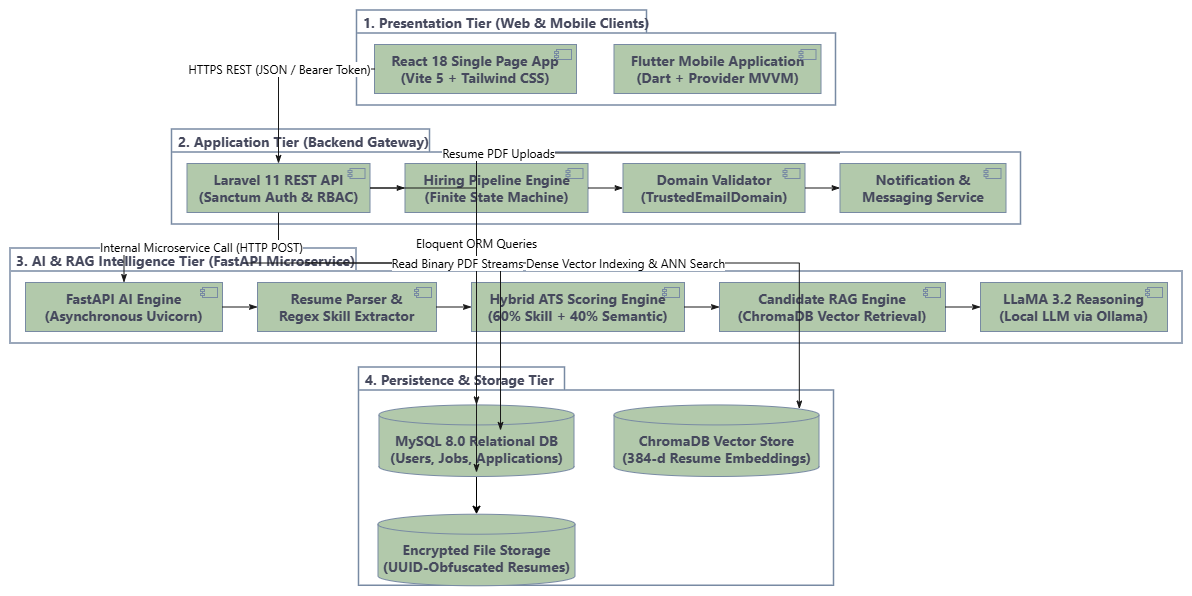
\includegraphics[width=0.9\linewidth]{figures/sys_architecture.png}
\caption{Decoupled Multi-Tier System Architecture of RecruitSense}
\label{fig:sys_arch_detail}
\end{figure}

\subsection{Frontend Layer}
The frontend is implemented on two distinct client platforms: a React and TypeScript Single Page Application (SPA) styled with Tailwind CSS, and a cross-platform mobile application engineered with Flutter and Dart. Both client implementations utilize type safety and deliver synchronized access to the recruitment ecosystem. The web client uses modern client-side routing via \texttt{react-router-dom} to deliver instant, fluid page transitions without full-page browser refreshes, while the mobile client implements the Model-View-ViewModel (MVVM) architecture with Provider-based reactive state management. Both platforms provide four distinct user surfaces:

\begin{itemize}
    \item \textbf{Public Job Discovery Surface:} Accessible to all visitors without requiring authentication. Visitors can browse active job listings, search vacancies by keyword or technology, filter by department, employment type (Full-Time, Part-Time, Remote, Contract), and salary range, and inspect detailed job descriptions. Implemented on both web and mobile platforms.
    \item \textbf{Authenticated Job Seeker Surface:} Available to registered candidates for profile and career experience management, PDF resume uploading, one-tap application submission with instant feedback, granular ATS match score visualization with skill gap breakdowns, curated learning course recommendations, personalized job bookmarks, and direct recruiter messaging. Implemented on both web and mobile platforms.
    \item \textbf{Recruiter and Employer Workspace Surface:} Equips verified corporate hiring managers with job vacancy creation and lifecycle management, candidate ranking tables sorted by computed ATS score, stage-by-stage hiring pipeline Kanban management, interactive Candidate RAG Q\&A dialogs with grounded resume citations, and interview calendar scheduling. Available on web and mobile with platform-optimized layouts.
    \item \textbf{Administrator Surface:} A restricted management interface for corporate email domain verification (\texttt{TrustedEmailDomain}), user and employer account moderation, job posting fraud review, global platform analytics, and audit logging. Implemented on the web platform due to the complex nature of governance tasks.
\end{itemize}

Both the web and mobile frontends are responsible for client-side form validation, guided multi-step workflows, contextual state updates, and centralized API token management via Axios and Dart HTTP interceptors. All security-critical authorization and state transitions are re-enforced server-side; the frontend layers serve strictly as user-facing interaction surfaces.

\subsection{Backend Application Layer}
The backend is implemented using Laravel 11 (PHP 8.2+). It serves as the authoritative central gateway for all business logic, data integrity, and workflow governance across the platform.

Core backend responsibilities include:
\begin{itemize}
    \item Authentication validation and token-based access control via Laravel Sanctum bearer tokens and Google OAuth 2.0.
    \item Role-Based Access Control (RBAC) middleware enforcing least-privilege route protection across \texttt{'job\_seeker'}, \texttt{'company'}, and \texttt{'admin'} user roles.
    \item Corporate email domain validation (\texttt{TrustedEmailDomain}) preventing unverified or disposable email registrations for employer accounts.
    \item Strict hiring pipeline state-machine enforcement (\textit{Applied} $\rightarrow$ \textit{Screening} $\rightarrow$ \textit{Shortlisted} $\rightarrow$ \textit{Interview} $\rightarrow$ \textit{Offer} $\rightarrow$ \textit{Rejected}).
    \item Real-time messaging orchestration, candidate notification dispatching, and application bookmark persistence.
    \item Secure internal HTTP integration with the computational Python FastAPI AI microservice.
\end{itemize}

A fundamental design principle is that all high-risk state transitions are validated server-side, guaranteeing that client applications cannot force invalid or unauthorized state modifications regardless of how HTTP requests are constructed.

\subsection{AI/ML and RAG Layer}
The artificial intelligence and conversational candidate intelligence service is an independent FastAPI application written in Python \cite{ramirez2019fastapi}. Decoupling the AI layer from the transactional PHP backend allows heavy machine learning model lifecycles, vector indexing, and GPU/CPU inference scaling to occur independently of core database operations.

AI capabilities integrated into RecruitSense include:
\begin{itemize}
    \item \textbf{PDF Document Text Extraction:} Asynchronously parses raw binary PDF streams page-by-page, strips binary encoding artifacts, and normalizes unstructured text.
    \item \textbf{Boundary-Delimited Skill Extraction:} Matches extracted resume text against an extensive multi-domain technology taxonomy, extracting matched competencies, identifying missing requirements, and capturing bonus skills.
    \item \textbf{Dense Semantic Vector Embedding:} Generates dense vector representations using sentence-transformer models (\texttt{all-MiniLM-L6-v2} and \texttt{nomic-embed-text}) to capture semantic relationships beyond exact keyword matches.
    \item \textbf{Candidate RAG Vector Search Engine:} Indexes chunked candidate resumes into persistent ChromaDB collections, allowing recruiters to perform conversational queries against candidate pools with grounded text citations and local LLM inference (LLaMA 3.2 via Ollama) \cite{lewis2020rag}.
    \item \textbf{Skill Gap Diagnostics and Course Recommendations:} Maps missing candidate technical competencies to curated educational courses and learning paths \cite{karimi2020course}.
    \item \textbf{Dynamic Assessment Quiz Generation:} Dynamically synthesizes customized multiple-choice technical assessment quizzes tailored to vacancy requirements.
\end{itemize}

\subsection{Data and Identity Layer}
RecruitSense utilizes MySQL 8.0 as its primary relational database management system alongside persistent disk-backed ChromaDB vector storage and secure local object storage. This layer provides strict data isolation, referential integrity, and forensic accountability for talent acquisition operations.

Concrete data services include:
\begin{itemize}
    \item \textbf{MySQL 8.0 Relational DBMS:} Stores structured domain entities including user credentials, company profiles, job vacancies, candidate applications, hiring pipeline stages, messages, notifications, and audit settings.
    \item \textbf{ChromaDB Vector Store:} Stores dense high-dimensional sentence embeddings of candidate resumes, supporting fast Hierarchical Navigable Small World (HNSW) approximate nearest neighbor vector searches.
    \item \textbf{Encrypted File Storage:} Object storage for candidate PDF resumes, profile images, and verification artifacts, stored outside the public web root with access restricted to authenticated controller streams.
\end{itemize}

Row-level authorization policies, foreign key constraints with cascading rules, and constraint-driven validation for status, role, and domain fields are strictly enforced throughout the database schema.

\subsection{Architectural Rationale}
The selected architecture is justified by five key rationale points:
\begin{enumerate}
    \item \textbf{Security-First Control:} Backend-owned state transitions, Sanctum token authentication, and corporate domain policy checks prevent client-side manipulation of critical hiring workflows on both web and mobile platforms.
    \item \textbf{Independent Multi-Tier Scalability:} The frontend clients (React and Flutter), transactional backend (Laravel), and AI inference microservice (FastAPI + ChromaDB) can each be scaled independently based on their respective CPU and memory demand profiles.
    \item \textbf{High Maintainability and Clean Boundaries:} Modular domain boundaries reduce the impact radius of code changes. Updating AI models or vector chunking algorithms does not disrupt transactional applicant records or authentication pipelines.
    \item \textbf{Explainable Trust Design:} Transparent ATS scoring formulations, missing skill badges, and grounded RAG citations eliminate black-box opacity, fostering trust among recruiters and candidates.
    \item \textbf{Cross-Platform Consistency:} A shared RESTful API client strategy ensures identical business logic enforcement, validation rules, and data structures across web and mobile surfaces.
\end{enumerate}

\section{Design Constraints}
This section presents the real constraints and assumptions that shaped design decisions throughout the development of RecruitSense.

\subsection{Technical Constraints}
\begin{itemize}
    \item \textbf{AI Inference Latency:} Machine learning inference and dense vector embedding operations are computationally demanding. PDF parsing and similarity scoring must execute within $2.0\text{ seconds}$, while RAG conversational candidate queries must return within $1.5\text{ seconds}$.
    \item \textbf{Resume Payload Size:} High-resolution PDF documents increase upload times and server memory consumption. Resume uploads are capped at a maximum of $5\text{MB}$ with client-side file type and MIME validation.
    \item \textbf{Mobile Frame Rate and Responsiveness:} Mobile UI rendering and animations must maintain a smooth 60 frames per second on standard consumer hardware, necessitating efficient asynchronous API fetching and local state caching.
    \item \textbf{CORS and Origin Isolation:} The decoupled frontend (React: Port 5173), mobile client, API backend (Laravel: Port 8000), and AI microservice (FastAPI: Port 8001) operate across distinct origins, requiring strict Cross-Origin Resource Sharing (CORS) origin validation and HTTPS header policies.
    \item \textbf{Workflow Determinism:} Candidate hiring states must be deterministic and transition-safe. Invalid state jumps (e.g., jumping from \textit{Applied} directly to \textit{Offer} without review) are rejected at the API layer.
\end{itemize}

\subsection{Data Constraints}
\begin{itemize}
    \item \textbf{Data Quality Dependency:} The accuracy of ATS match scoring and candidate ranking is directly dependent on the readability and text clarity of candidate-uploaded PDF resumes.
    \item \textbf{Schema Evolution and Backward Compatibility:} Database migrations must preserve historical applicant records and maintain compatibility across active mobile app versions.
    \item \textbf{Search Normalization:} User job search queries and skill inputs are often noisy and inconsistently formatted, requiring string trimming, case normalization, and taxonomy synonym mapping.
    \item \textbf{Evidence Traceability:} All application state changes, interview records, and domain verifications require durable foreign key references and timestamps for governance accountability.
\end{itemize}

\subsection{Security and Compliance Constraints}
\begin{itemize}
    \item \textbf{Least-Privilege Principle:} Privileged administrative and recruiter actions are strictly scoped to verified user IDs and authorized role permissions via Laravel middleware.
    \item \textbf{Sensitive Document Privacy:} Candidate resumes contain personally identifiable information (PII) and must remain in private, access-controlled storage accessible only by the applicant and authorized hiring managers.
    \item \textbf{Auditability:} All corporate domain approvals, account suspensions, and content moderation overrides must produce durable audit trail records in the database.
    \item \textbf{Abuse Prevention and Rate Limiting:} High-frequency endpoints, including AI screening triggers, login attempts, and job application submissions, are protected against brute-force attacks via API throttling and rate limiting.
\end{itemize}

\subsection{Product and Business Constraints}
\begin{itemize}
    \item \textbf{Trust-First Recruitment Ecosystem:} Corporate recruitment requires verified employer identities to eliminate fake listings, phishing scams, and fraudulent job postings.
    \item \textbf{Friction Budget:} Candidate workflows must remain frictionless while enforcing necessary validation, ensuring high application completion rates without sacrificing screening fidelity.
    \item \textbf{Feature-Tier Growth:} The architecture is designed to support future enterprise monetization tiers, advanced coding sandbox assessments, and external job board syndication without core database restructuring.
\end{itemize}

\subsection{Operational Constraints}
\begin{itemize}
    \item \textbf{Multi-Service Deployment:} Frontend web hosting, backend API hosting, and Python AI service hosting may reside across different virtualized server environments, requiring environment-aware configuration management via \texttt{.env} files.
    \item \textbf{Monitoring Maturity:} System health is monitored via structured logging, HTTP status monitoring, and health check endpoints on both API and AI microservices.
    \item \textbf{Incident Diagnosis:} Comprehensive error handling and correlation IDs facilitate rapid diagnosis of inter-service communication issues.
\end{itemize}

\subsection{Assumptions}
\begin{itemize}
    \item Users possess standard digital literacy sufficient to navigate web and mobile application interfaces.
    \item Job seekers provide authentic resume data, and employers post legitimate employment terms.
    \item Administrative users adhere to standard moderation operating procedures and ethical guidelines.
    \item Uploaded PDF resumes contain extractable text layers rather than scanned flat bitmap images.
\end{itemize}

\section{Design Methodology}
RecruitSense was engineered using a hybrid methodology combining incremental domain delivery, layered separation of concerns, and finite state-machine modeling for critical operational workflows \cite{sommerville2016software}.

\subsection{Incremental Domain Delivery}
The platform was developed across five functional increments, with each increment delivering complete vertical end-to-end functionality spanning presentation, API, and persistence layers:
\begin{enumerate}
    \item \textbf{Core Identity and Role-Governed Access:} User registration, corporate domain validation, Sanctum token authentication, and role assignment.
    \item \textbf{Job Vacancy Lifecycle and Candidate Application:} Job posting creation, search and filtering, resume upload, and transactional application persistence.
    \item \textbf{AI Screening and RAG Intelligence:} PDF text extraction, boundary-delimited skill matching, ATS score computation, ChromaDB vector indexing, and conversational candidate querying.
    \item \textbf{Candidate Management and Communication:} Recruiter applicant review tables, hiring pipeline stage progression, interview scheduling, and real-time in-app messaging.
    \item \textbf{Community Networking and Governance:} Professional networking feed, job bookmarking, content moderation, domain approval queues, and system analytics.
\end{enumerate}

\subsection{Layered Separation of Concerns}
The architecture enforces strict separation of concerns: the client layer handles user interface rendering and interaction; the backend API layer owns business rules, input validation, and transactional persistence; the AI microservice layer owns model inference and semantic vector matching; and the data layer owns data integrity, relational constraints, and vector persistence.

\subsection{State-Machine Methodology for Critical Workflows}
Critical recruitment modules were explicitly modeled as formal Finite State Machines (FSMs) with defined legal transitions. The candidate hiring pipeline is governed by the state machine depicted in Figure \ref{fig:fsm_pipeline}, ensuring that applications progress strictly through valid states (\textit{Applied} $\rightarrow$ \textit{Screening} $\rightarrow$ \textit{Shortlisted} $\rightarrow$ \textit{Interview} $\rightarrow$ \textit{Offer} or \textit{Rejected}). This prevents race conditions and illegal status modifications.

\begin{figure}[H]
\centering
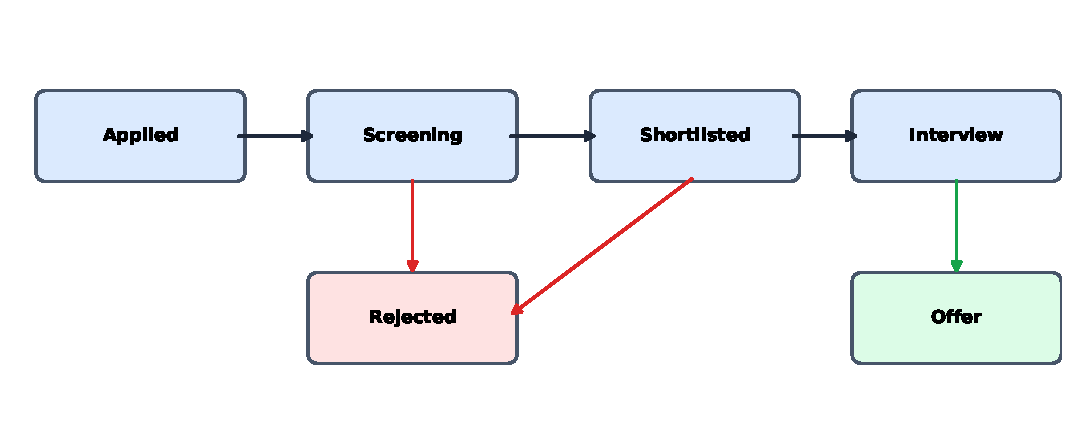
\includegraphics[width=0.8\linewidth]{figures/hiring_fsm.pdf}
\caption{Finite State Machine for Candidate Hiring Pipeline}
\label{fig:fsm_pipeline}
\end{figure}

\subsection{Threat-Aware Design Methodology}
Security was integrated into system design from the outset. Anticipated threats—such as resume keyword stuffing, unauthorized status tampering, disposable domain abuse, and insecure direct object references—were mitigated through embedded architectural controls including boundary-delimited taxonomy extraction, server-side RBAC middleware, and token-authenticated document streams \cite{owasp2021top10}.

\subsection{Design-for-Change Strategy}
The platform is structured to support evolving technology standards. The AI service uses modular interfaces allowing embedding models (\texttt{all-MiniLM-L6-v2}, \texttt{nomic-embed-text}) or LLM backends (Ollama, local vLLM) to be swapped without requiring changes to the frontend or database schemas.

\section{High-Level Block Diagram}
RecruitSense can be abstracted into four major functional blocks that correspond to the four architectural layers described in Section 4.1.

\begin{figure}[H]
\centering
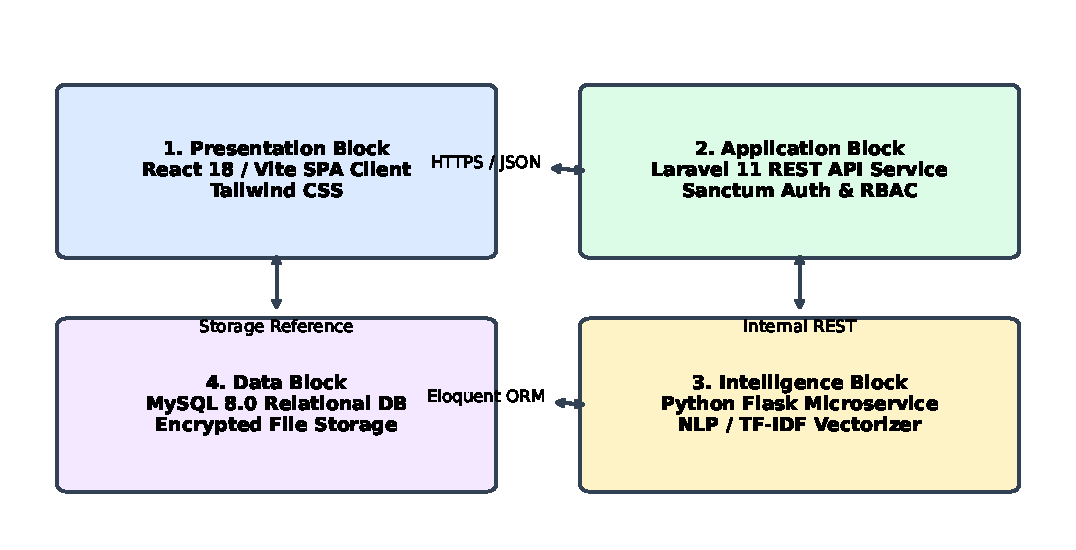
\includegraphics[width=0.8\linewidth]{figures/block_diagram.pdf}
\caption{High-Level Functional Block Diagram of RecruitSense}
\label{fig:high_level_blocks}
\end{figure}

The four functional blocks operate synchronously and asynchronously:
\begin{enumerate}
    \item \textbf{Presentation Block (React Web \& Flutter Mobile):} Handles user interactions, form validation, dynamic state rendering, and API communication.
    \item \textbf{Application Layer (Laravel 11 REST API):} Enforces business logic, handles authentication and RBAC, executes database CRUD operations, and coordinates service workflows.
    \item \textbf{AI/ML Layer (FastAPI Microservice):} Conducts PDF text parsing, taxonomy matching, dense semantic embedding, ChromaDB vector querying, dynamic quiz generation, and course recommendations.
    \item \textbf{Data Layer (MySQL 8.0 Relational DBMS + ChromaDB + File Storage):} Persists relational tables, dense vector embeddings, and encrypted resume files.
\end{enumerate}

\section{Low-Level Design: System Sequence Diagrams (SSDs)}
This section presents the System Sequence Diagrams (SSDs) for the core functional workflows of RecruitSense, detailing the sequence of message exchanges, parameter transfers, database queries, and state transitions between actors and subsystems.

\subsection{SSD-01: Browse and Filter Jobs}
As described in Figure \ref{fig:ssd01}, when a user visits the RecruitSense platform on web or mobile, they interact with the job exploration interface to discover employment opportunities. The user enters search keywords (e.g., job title, domain keywords, or required skills) and selects optional filtering parameters such as employment type (Full-time, Part-time, Remote, Contract), minimum salary range, and department category. The frontend client dispatches an HTTP GET request with serialized query parameters to the Laravel API endpoint \texttt{/api/jobs}. The backend controller validates the parameters and executes an optimized SQL query against the \texttt{job\_postings} table with active status constraints and eager-loaded company relationships. The retrieved collection of active vacancies is serialized into JSON and returned to the client with an HTTP 200 OK status. The frontend dynamically renders the matching job cards, displaying company metadata, salary badges, and required skills without requiring full-page reloads. When the user selects a specific job card, the full vacancy description and qualifications are rendered in a detailed modal.

\begin{figure}[H]
\centering
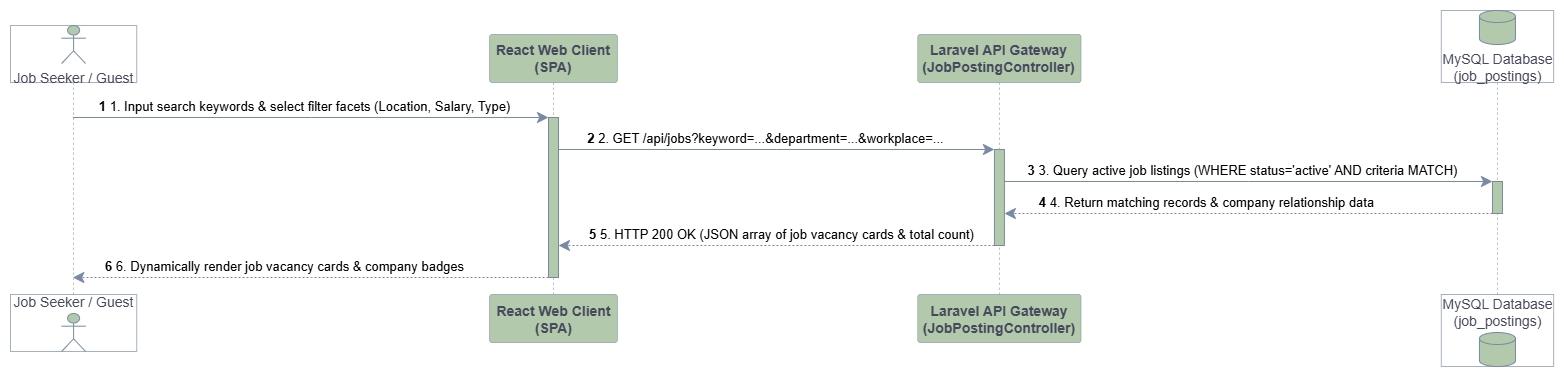
\includegraphics[width=0.75\linewidth]{figures/ssd_01.png}
\caption{Browse and Filter Jobs Sequence Diagram}
\label{fig:ssd01}
\end{figure}

\subsection{SSD-02: Register User with Role Assignment}
As described in Figure \ref{fig:ssd02}, when a new user registers on RecruitSense, they complete the registration form on the web or mobile client by providing their full name, email address, password, and selecting their account role (\textit{Job Seeker} or \textit{Employer/Company}). The client performs client-side field validation and submits an HTTP POST request to \texttt{/api/register}. The Laravel backend verifies that the email address is unique in the \texttt{users} table. If the selected role is \textit{Company}, the custom \texttt{TrustedEmailDomain} validation rule verifies that the email domain is an authentic enterprise domain rather than a free or disposable provider (e.g., rejecting \texttt{@gmail.com} or \texttt{@tempmail.com}). Once validated, the system hashes the password using Bcrypt (12 rounds), inserts the new record into the \texttt{users} table, creates the corresponding profile record in \texttt{job\_seekers} or \texttt{companies}, issues a personal access token via Laravel Sanctum, and returns the token with user metadata. The client stores the token securely and redirects the user to their role-specific onboarding dashboard.

\begin{figure}[H]
\centering
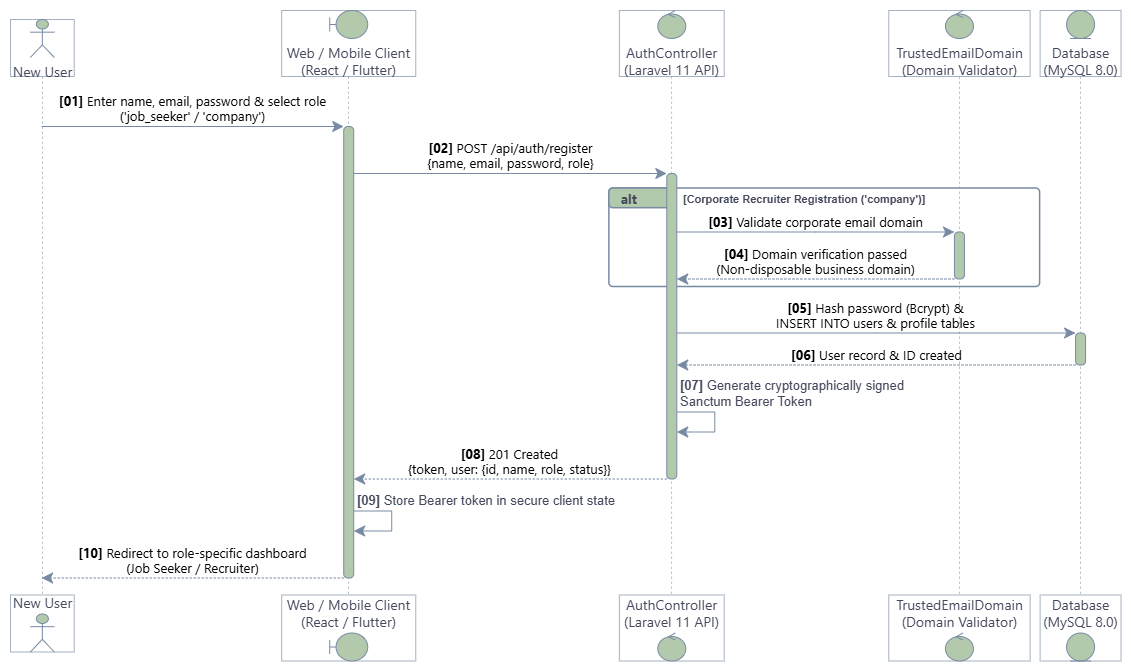
\includegraphics[width=0.75\linewidth]{figures/ssd_02.png}
\caption{Register User with Role Assignment Sequence Diagram}
\label{fig:ssd02}
\end{figure}

\subsection{SSD-03: User Login and Token Authentication}
As described in Figure \ref{fig:ssd03}, an existing user initiates authentication by entering their registered email address and password on the login screen, or by initiating Google OAuth Single Sign-On. The client submits an HTTP POST request to \texttt{/api/login}. The backend queries the \texttt{users} table by email, checks if the account is active and not suspended, and verifies the entered password against the stored Bcrypt hash using secure constant-time comparison. Upon successful verification, expired tokens are pruned, a fresh Laravel Sanctum personal access token is issued with role-scoped abilities, and the user's role and profile data are returned in the response payload. The client stores the bearer token in local storage or secure mobile storage, configures default authorization headers for subsequent requests, and navigates the user to their personalized workspace.

\begin{figure}[H]
\centering
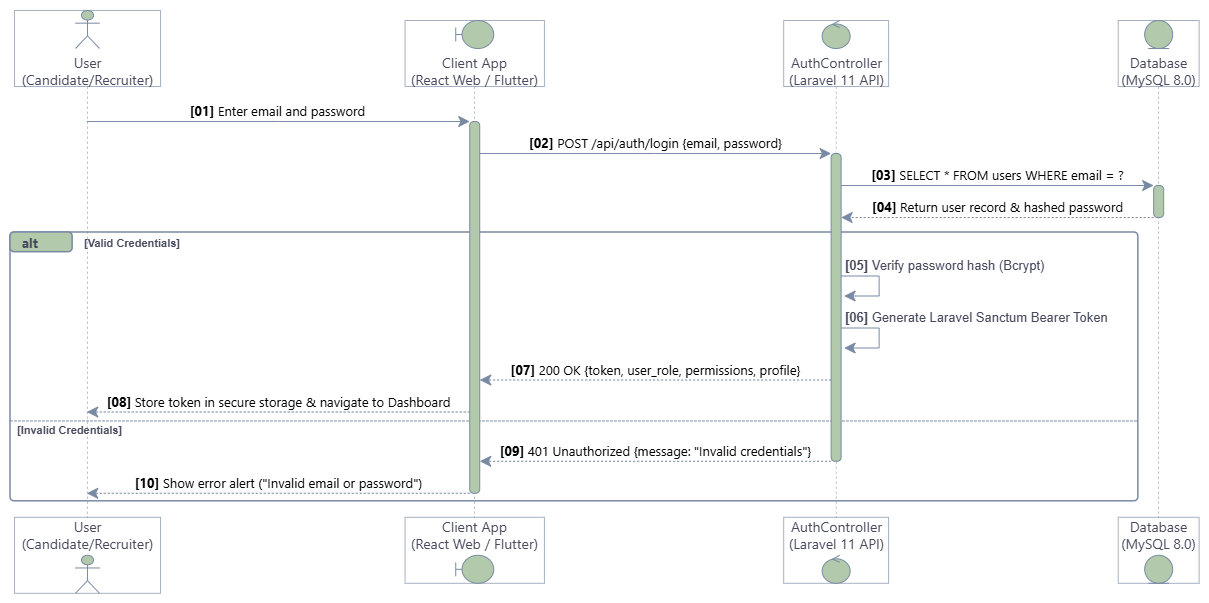
\includegraphics[width=0.75\linewidth]{figures/ssd_03.png}
\caption{User Login and Token Authentication Sequence Diagram}
\label{fig:ssd03}
\end{figure}

\subsection{SSD-04: Create and Publish Job Vacancy}
As described in Figure \ref{fig:ssd04}, a verified corporate recruiter creates a new job opening by accessing the vacancy creator form. The recruiter enters the job title, department, employment type, location, salary range, comprehensive description, and a comma-separated list of required technical skills. Upon form submission, the frontend sends an authenticated HTTP POST request to \texttt{/api/jobs} with the Sanctum bearer token. The backend middleware verifies that the user holds the \texttt{'company'} role and that their corporate domain is verified. The controller validates all input fields, sanitizes HTML description tags, inserts the record into the \texttt{job\_postings} table with an initial status of \texttt{'active'}, and records the associated \texttt{company\_id}. The newly created job object is returned to the client, and the recruiter dashboard updates its active job list.

\begin{figure}[H]
\centering
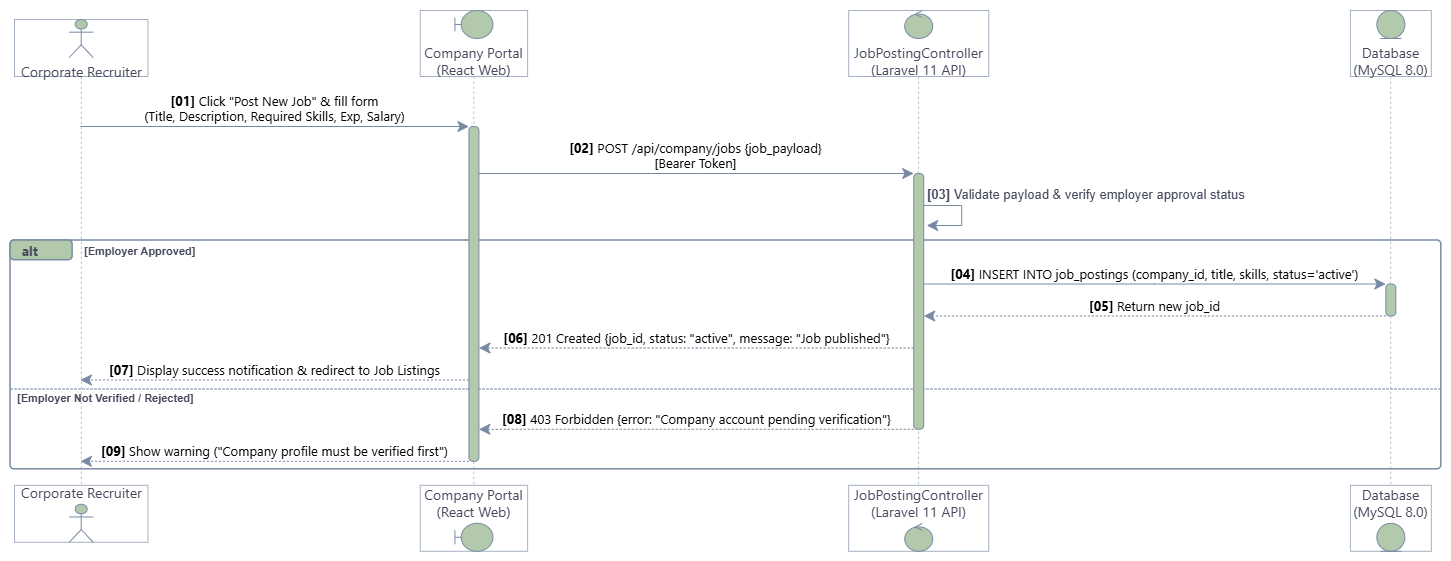
\includegraphics[width=0.75\linewidth]{figures/ssd_04.png}
\caption{Create and Publish Job Vacancy Sequence Diagram}
\label{fig:ssd04}
\end{figure}

\subsection{SSD-05: Submit Job Application and Automated AI Screening}
As described in Figure \ref{fig:ssd05}, an authenticated job seeker applies for an open position by uploading their PDF resume through the application modal. The client packages the multipart/form-data payload and dispatches an HTTP POST request to \texttt{/api/applications}. The Laravel backend validates file type (\texttt{application/pdf}) and size ($\le 5\text{MB}$), stores the resume file in a private storage directory with an obfuscated UUID filename, and immediately triggers an internal HTTP call to the FastAPI AI microservice endpoint \texttt{/api/v1/extract-and-score}. The AI microservice parses the PDF text layer, executes boundary-delimited skill matching against the job's required skills, calculates keyword and semantic match percentages, generates dense sentence embeddings, and indexes the resume chunks into ChromaDB. The AI service returns the computed ATS match score ($0\text{--}100\%$), matched skills, missing skills, and course recommendations. The backend persists the application in the \texttt{applications} table and the detailed skill breakdown in \texttt{skill\_gaps}, and returns the complete evaluation to the candidate with real-time visual feedback.

\begin{figure}[H]
\centering
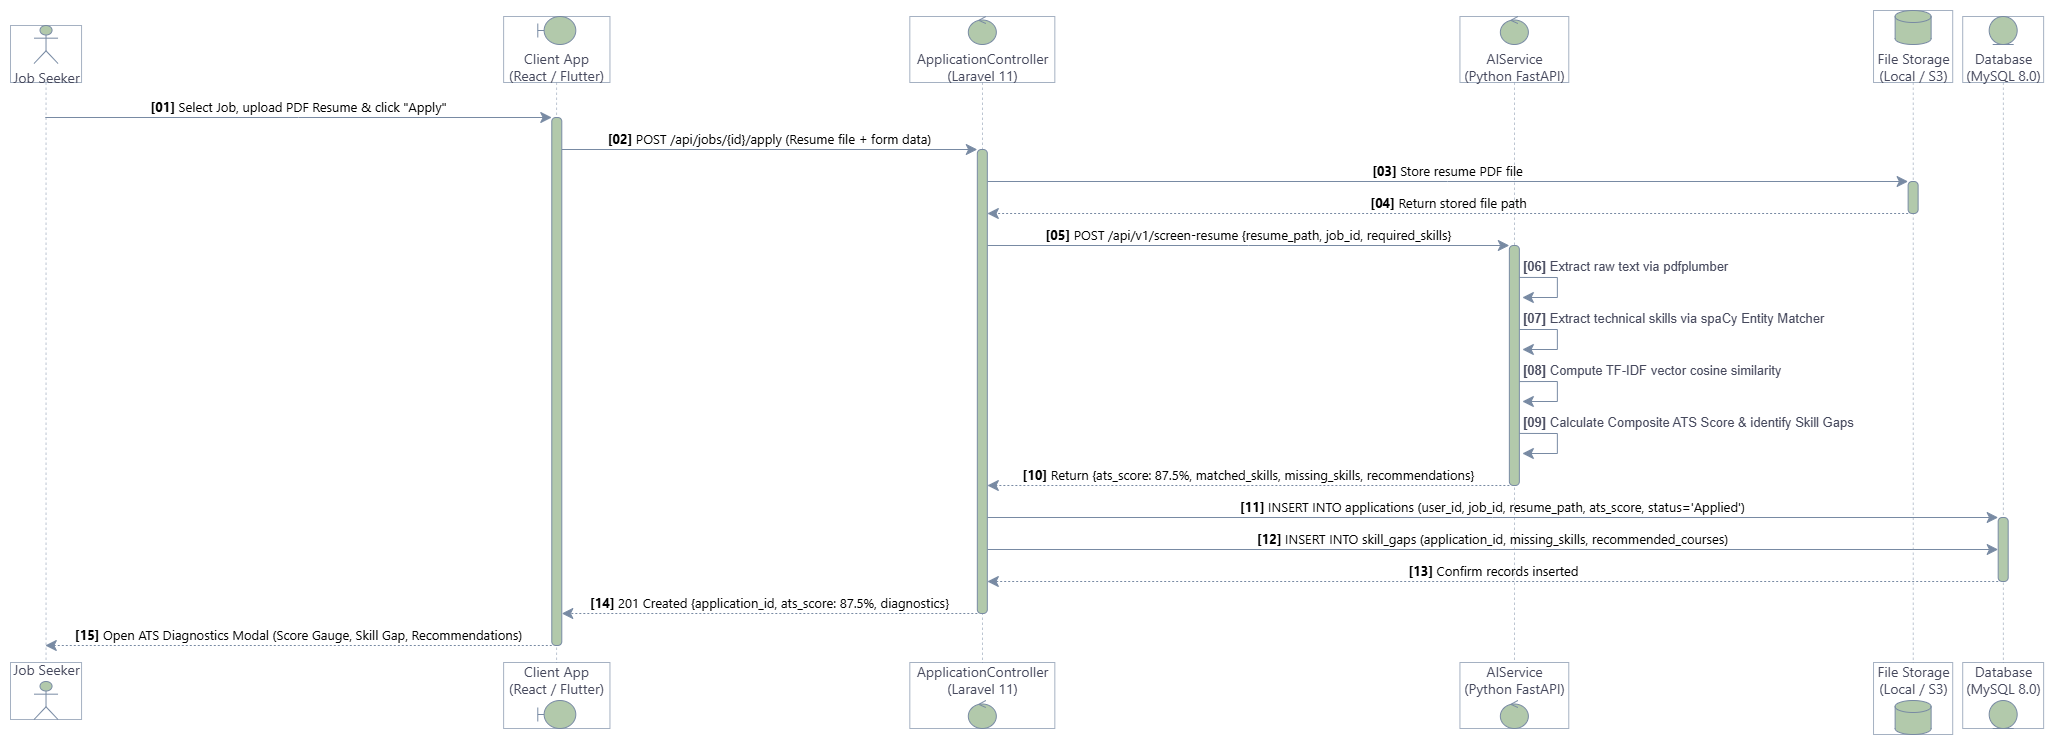
\includegraphics[width=0.75\linewidth]{figures/ssd_05.png}
\caption{Submit Job Application and Automated AI Screening Sequence Diagram}
\label{fig:ssd05}
\end{figure}

\subsection{SSD-06: Review AI-Ranked Candidate Shortlist}
As described in Figure \ref{fig:ssd06}, a recruiter reviews the applicant pool for a specific job vacancy by navigating to the applicant manager. The frontend sends an authenticated GET request to \texttt{/api/jobs/\{id\}/applications}. The backend verifies that the requesting recruiter owns the job posting, queries the \texttt{applications} table joined with \texttt{job\_seekers} and \texttt{skill\_gaps}, and orders the candidate records in descending order of computed \texttt{ats\_score}. The response returns the ranked candidate list with matched skills, missing skills, and application status. The recruiter interface renders an interactive ranking table with color-coded ATS badges, allowing the recruiter to filter by score thresholds, inspect individual candidate profiles, open secure resume previews, or launch conversational Candidate RAG dialogs.

\begin{figure}[H]
\centering
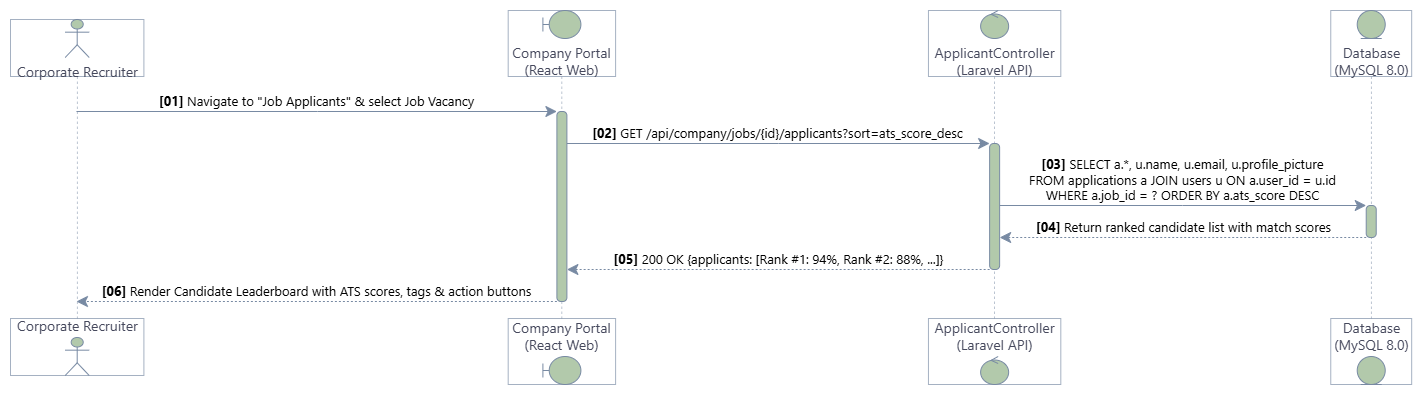
\includegraphics[width=0.75\linewidth]{figures/ssd_06.png}
\caption{Review AI-Ranked Candidate Shortlist Sequence Diagram}
\label{fig:ssd06}
\end{figure}

\subsection{SSD-07: Manage Hiring Pipeline Status}
As described in Figure \ref{fig:ssd07}, a hiring manager updates the progression stage of a candidate within the hiring pipeline (e.g., advancing from \textit{Applied} to \textit{Shortlisted}, \textit{Interview}, \textit{Offer}, or \textit{Rejected}). The recruiter drags a candidate card on the Kanban board or selects a new status from a dropdown menu. The client sends an HTTP PATCH request to \texttt{/api/applications/\{id\}/status} containing the target status. The backend verifies authorization and executes state-machine validation to ensure the transition is legally permitted according to the hiring FSM. Upon validation, the backend updates the \texttt{status} column in the \texttt{applications} table, logs the transition timestamp, and automatically queues an in-app and email notification to the candidate. The updated application object is returned, and both the recruiter Kanban board and candidate application tracker reflect the new status.

\begin{figure}[H]
\centering
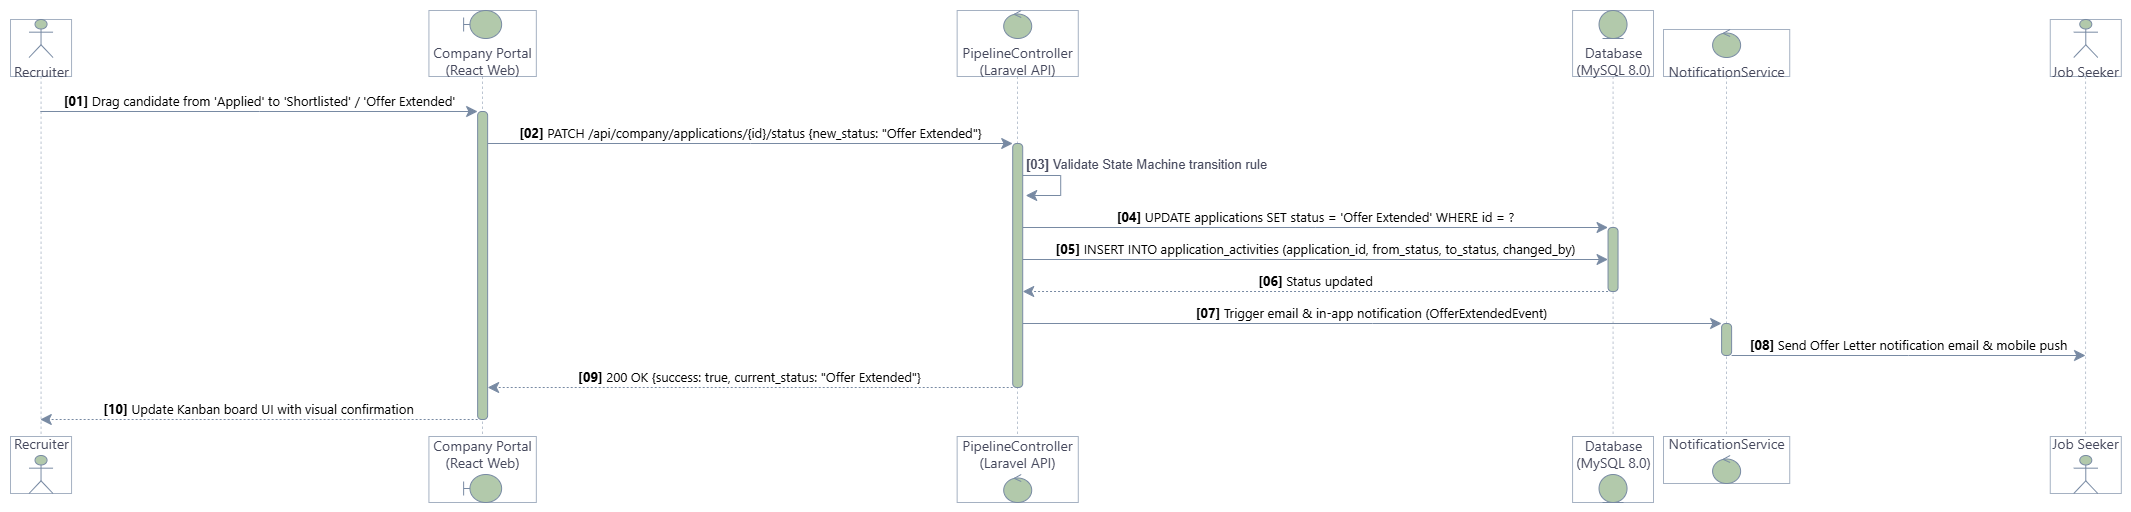
\includegraphics[width=0.75\linewidth]{figures/ssd_07.png}
\caption{Manage Hiring Pipeline Status Sequence Diagram}
\label{fig:ssd07}
\end{figure}

\subsection{SSD-08: Schedule Candidate Interview}
As described in Figure \ref{fig:ssd08}, a recruiter schedules an interview with a shortlisted candidate by selecting the interview action on the candidate's application card. The recruiter fills in the date, time, interview format (In-Person, Video Call), and optional meeting URL or notes, and clicks submit. The client sends an HTTP POST request to \texttt{/api/applications/\{id\}/schedule-interview}. The backend verifies employer ownership, validates that the date is set in the future, updates the \texttt{interview\_at} timestamp and application status to \textit{Interview} in the \texttt{applications} table, and inserts an interview notification into the \texttt{notifications} table. The candidate receives an instant alert with interview details and calendar integration links on both web and mobile workspaces.

\begin{figure}[H]
\centering
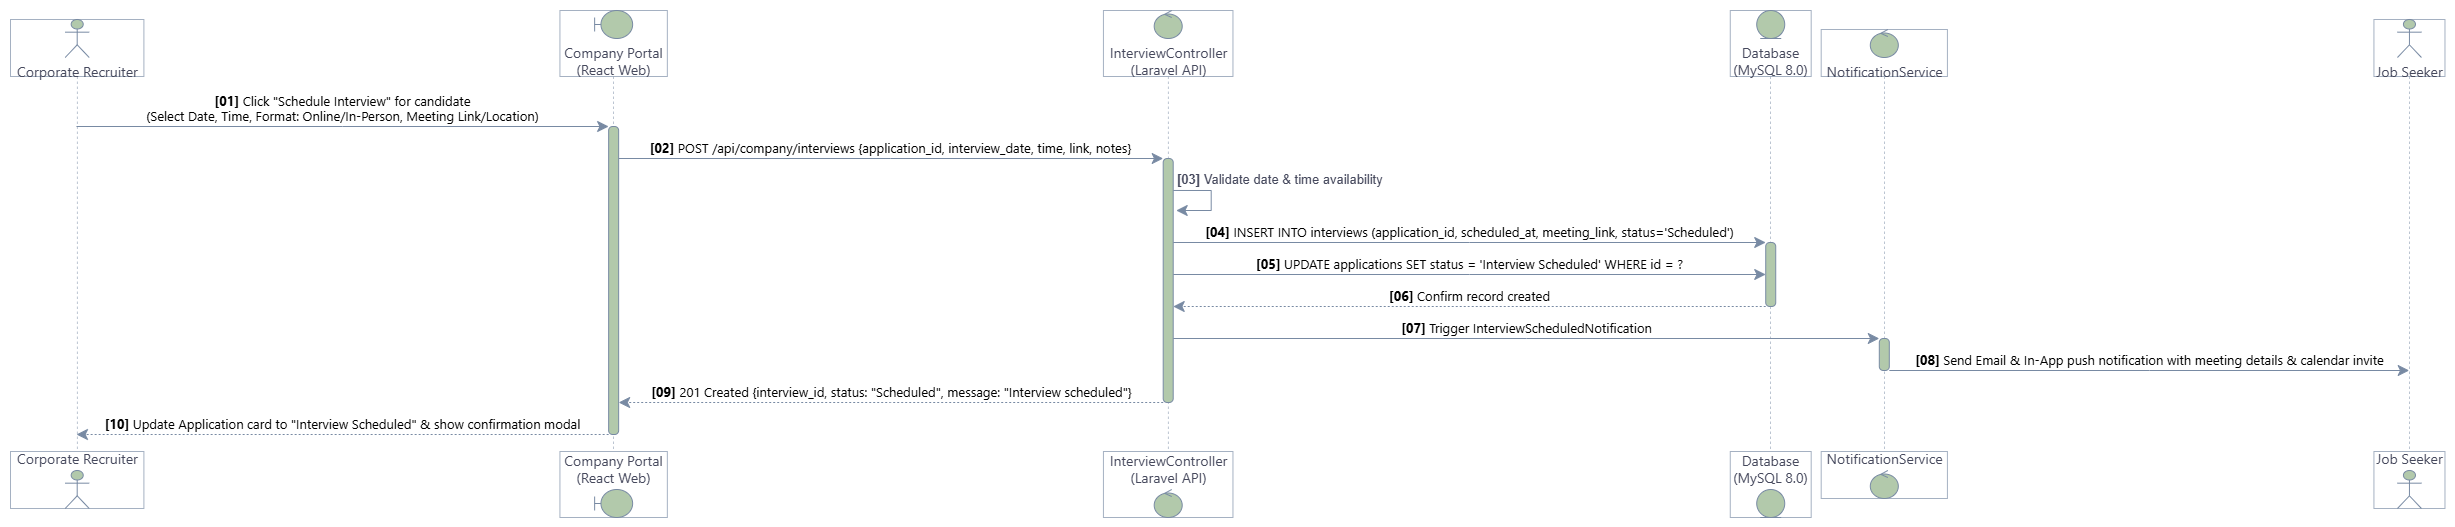
\includegraphics[width=0.75\linewidth]{figures/ssd_08.png}
\caption{Schedule Candidate Interview Sequence Diagram}
\label{fig:ssd08}
\end{figure}

\subsection{SSD-09: Real-Time In-App Messaging}
As described in Figure \ref{fig:ssd09}, a job seeker and recruiter engage in direct in-app messaging to discuss application details and interview coordination. When the sender types a message and clicks send, the client sends an authenticated POST request to \texttt{/api/messages} with the recipient ID, conversation ID, and message text. The backend verifies that the sender belongs to the conversation, sanitizes the message content against XSS vulnerabilities, inserts the record into the \texttt{messages} table, updates the conversation's \texttt{updated\_at} timestamp, and returns the message payload. The recipient's active client receives the message in real time, updating the chat dialog dynamically without requiring page refreshes.

\begin{figure}[H]
\centering
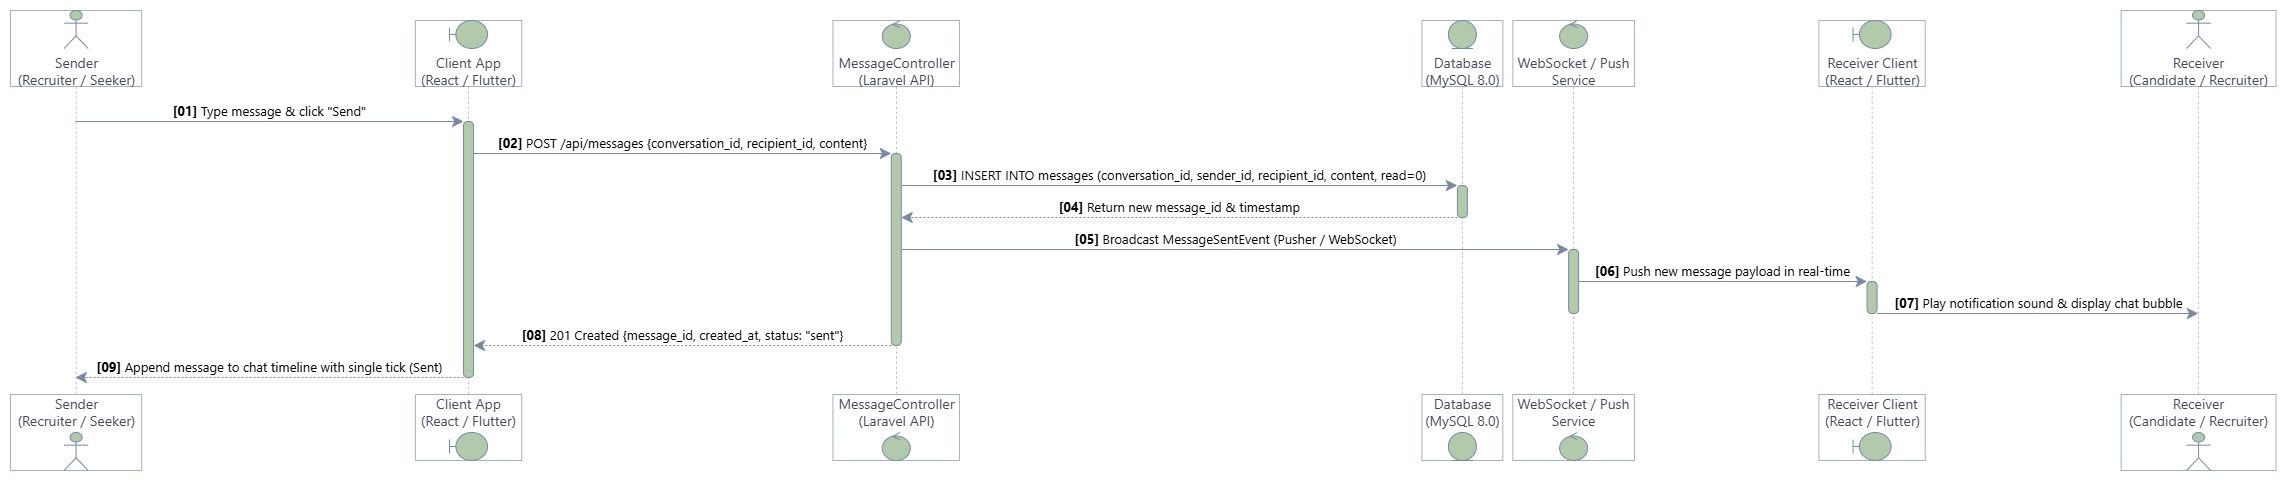
\includegraphics[width=0.75\linewidth]{figures/ssd_09.png}
\caption{Real-Time In-App Messaging Sequence Diagram}
\label{fig:ssd09}
\end{figure}

\subsection{SSD-10: Verify Corporate Email Domain (Admin)}
As described in Figure \ref{fig:ssd10}, a platform administrator manages the trust governance queue by reviewing pending corporate employer email domains. The administrator accesses the admin console, sending a GET request to \texttt{/api/admin/domains/pending}. The backend verifies administrator RBAC permissions and retrieves unverified domain records from \texttt{companies}. The administrator inspects corporate documentation and clicks ``Approve Domain''. The client dispatches a POST request to \texttt{/api/admin/domains/\{id\}/approve}. The backend updates the company's \texttt{verified} flag to \texttt{true}, logs the administrative decision in the audit log, and dispatches an approval notification to the employer, enabling full job posting and applicant screening capabilities.

\begin{figure}[H]
\centering
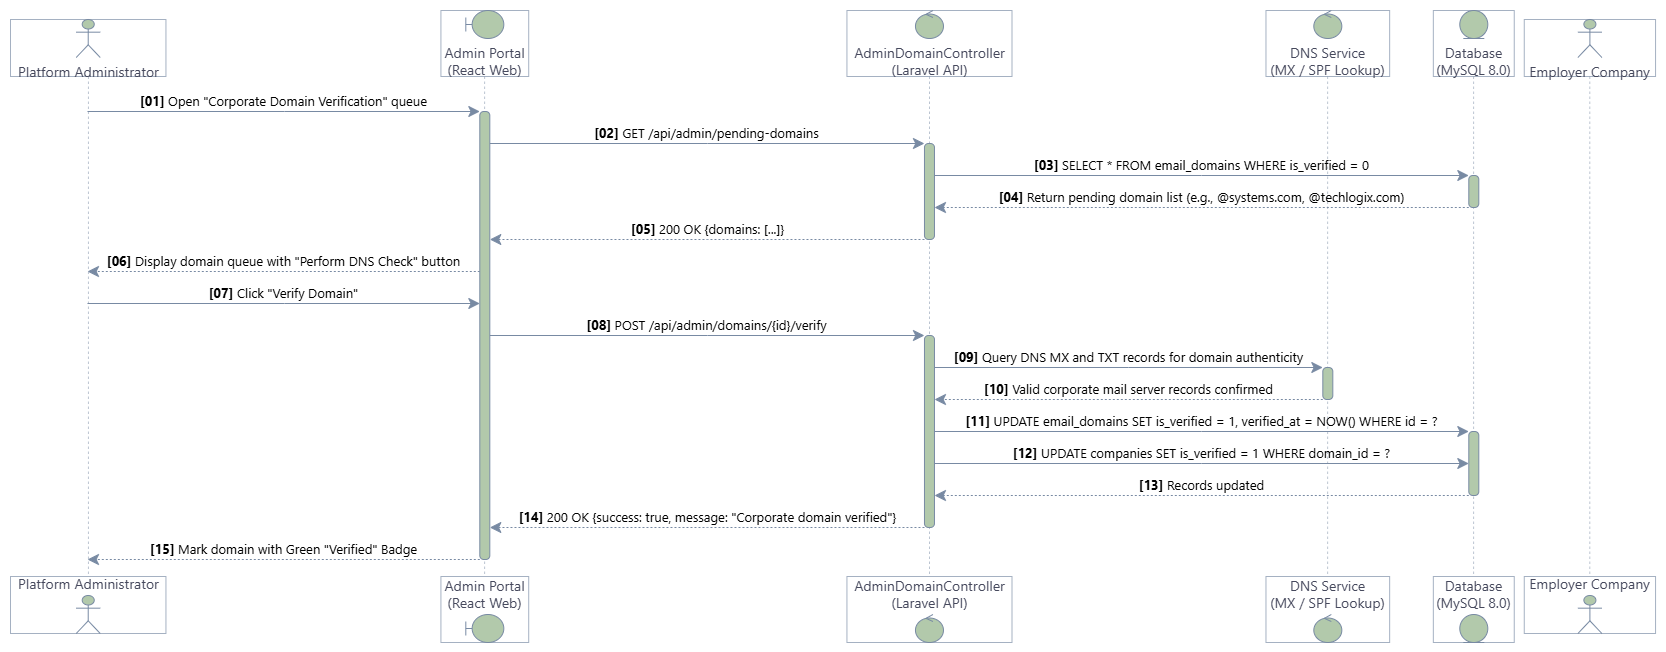
\includegraphics[width=0.75\linewidth]{figures/ssd_10.png}
\caption{Verify Corporate Email Domain Sequence Diagram}
\label{fig:ssd10}
\end{figure}

\subsection{SSD-11: Save Job to Bookmarks}
As described in Figure \ref{fig:ssd11}, an authenticated job seeker bookmarks an interesting job listing for future review by clicking the bookmark icon on any job card. The client issues an HTTP POST request to \texttt{/api/jobs/\{id\}/save}. The backend validates the candidate's session token, verifies that the target job exists, checks for existing bookmark entries, and inserts a new record into the \texttt{saved\_jobs} table with the user ID and job posting ID. The API returns a success response, and the client updates the bookmark icon state to active. If the user clicks the bookmark icon again, a DELETE request is dispatched, removing the record and updating the UI state accordingly.

\begin{figure}[H]
\centering
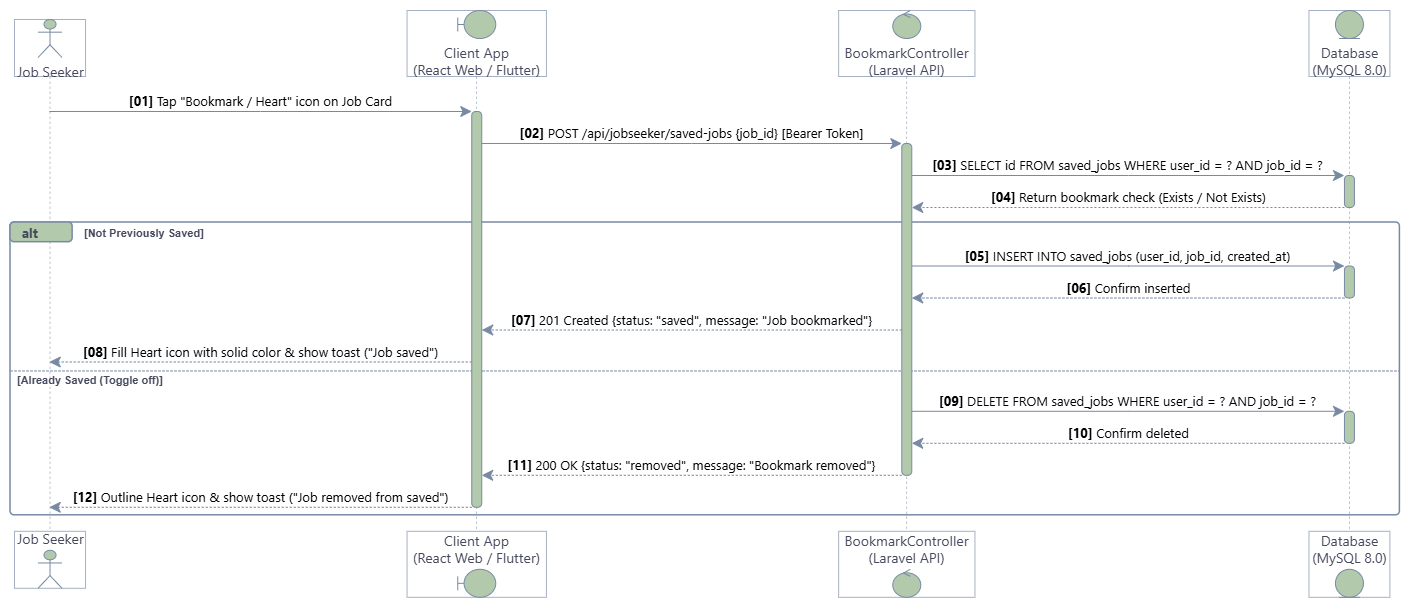
\includegraphics[width=0.75\linewidth]{figures/ssd_11.png}
\caption{Save Job to Bookmarks Sequence Diagram}
\label{fig:ssd11}
\end{figure}

\subsection{SSD-12: Edit and Update Job Vacancy}
As described in Figure \ref{fig:ssd12}, a corporate employer modifies an existing job opening by navigating to the job editor interface. The employer updates job details---such as description, salary range, or required skill taxonomy---and submits the form. The client dispatches an HTTP PUT request to \texttt{/api/jobs/\{id\}}. The backend middleware confirms that the requesting user owns the job posting, validates updated input fields, and updates the corresponding record in the \texttt{job\_postings} table. The updated job record is returned to the client, and the active vacancy listing is updated across public browsing surfaces.

\begin{figure}[H]
\centering
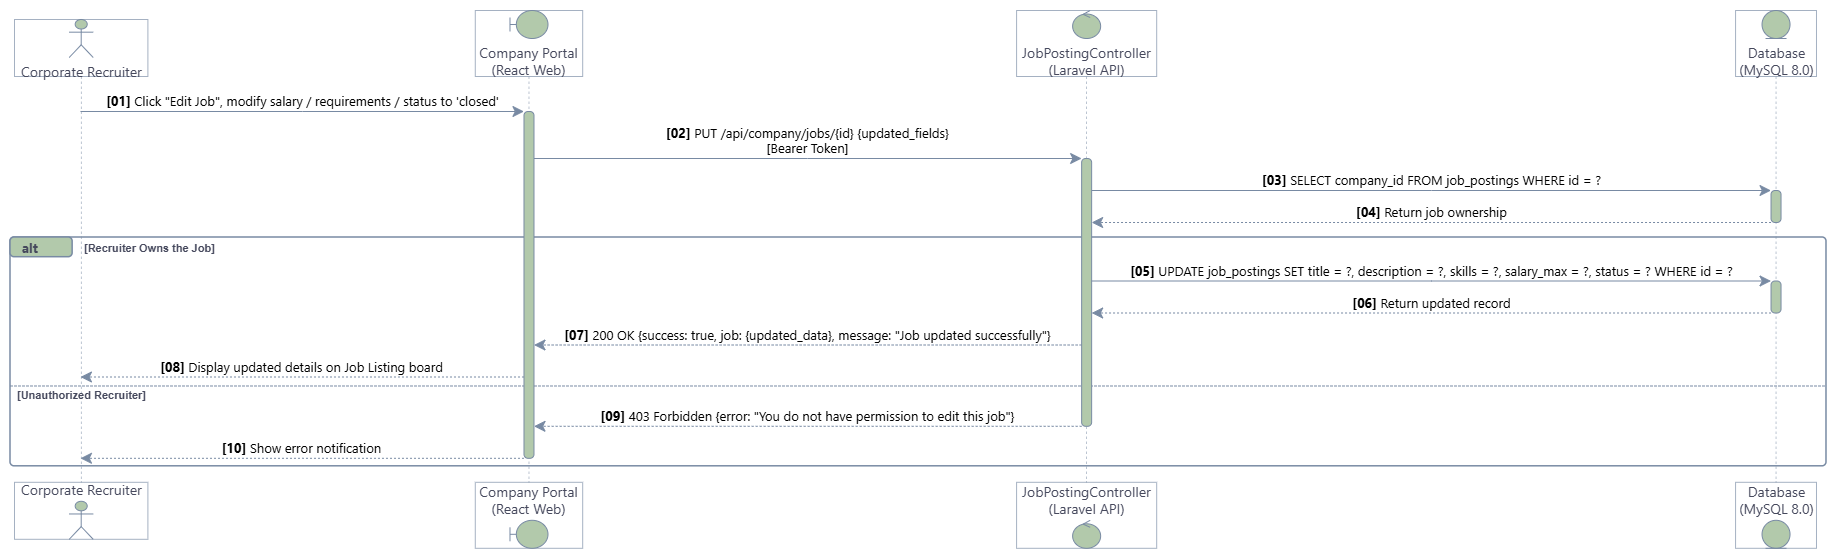
\includegraphics[width=0.75\linewidth]{figures/ssd_12.png}
\caption{Edit and Update Job Vacancy Sequence Diagram}
\label{fig:ssd12}
\end{figure}

\subsection{SSD-13: Moderate Employer Accounts}
As described in Figure \ref{fig:ssd13}, a system administrator oversees corporate compliance by inspecting registered employer profiles in the moderation console. When an employer account exhibits suspicious behavior or reports of fraudulent postings, the administrator reviews the company profile, verified domain status, and active vacancies. The administrator can approve, flag, or suspend the employer account by sending an HTTP POST request to \texttt{/api/admin/companies/\{id\}/status} with the action and moderation notes. The backend updates the company status, suspends associated active job listings if necessary, records an audit log entry, and issues an account status email to the employer.

\begin{figure}[H]
\centering
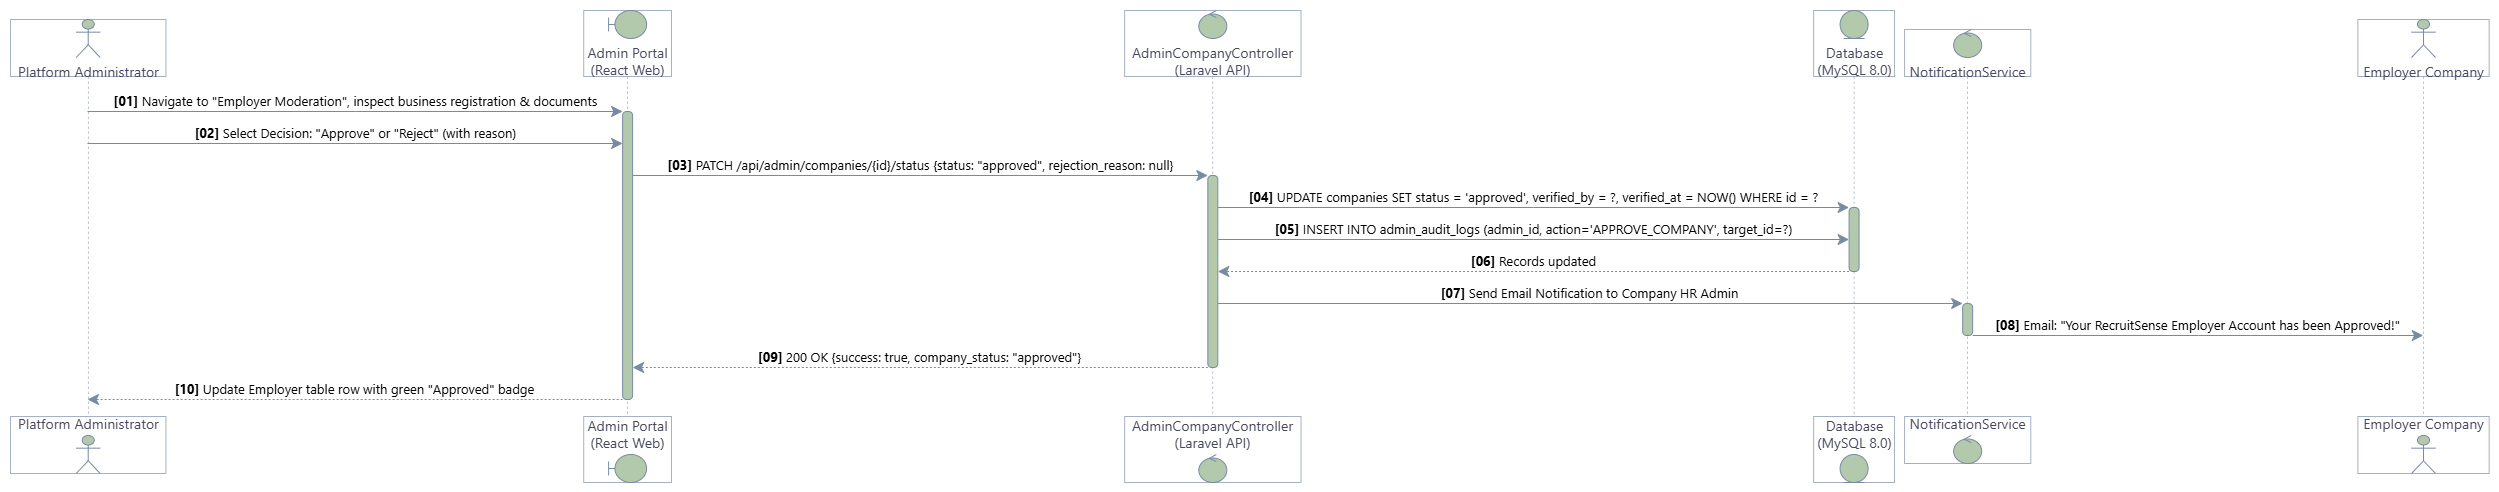
\includegraphics[width=0.75\linewidth]{figures/ssd_13.png}
\caption{Moderate Employer Accounts Sequence Diagram}
\label{fig:ssd13}
\end{figure}

\subsection{SSD-14: Moderate User Accounts and Suspensions}
As described in Figure \ref{fig:ssd14}, a system administrator manages user compliance and enforces platform community guidelines. The administrator searches for a reported user account in the user management panel, inspects their profile history and reported infractions, and selects a moderation action (Issue Warning, Temporary Suspension, or Permanent Ban). The client submits an HTTP POST request to \texttt{/api/admin/users/\{id\}/moderate}. The backend validates administrator privileges, updates the \texttt{status} column in the \texttt{users} table, revokes all active Sanctum bearer tokens for the affected user, and creates a persistent moderation audit record.

\begin{figure}[H]
\centering
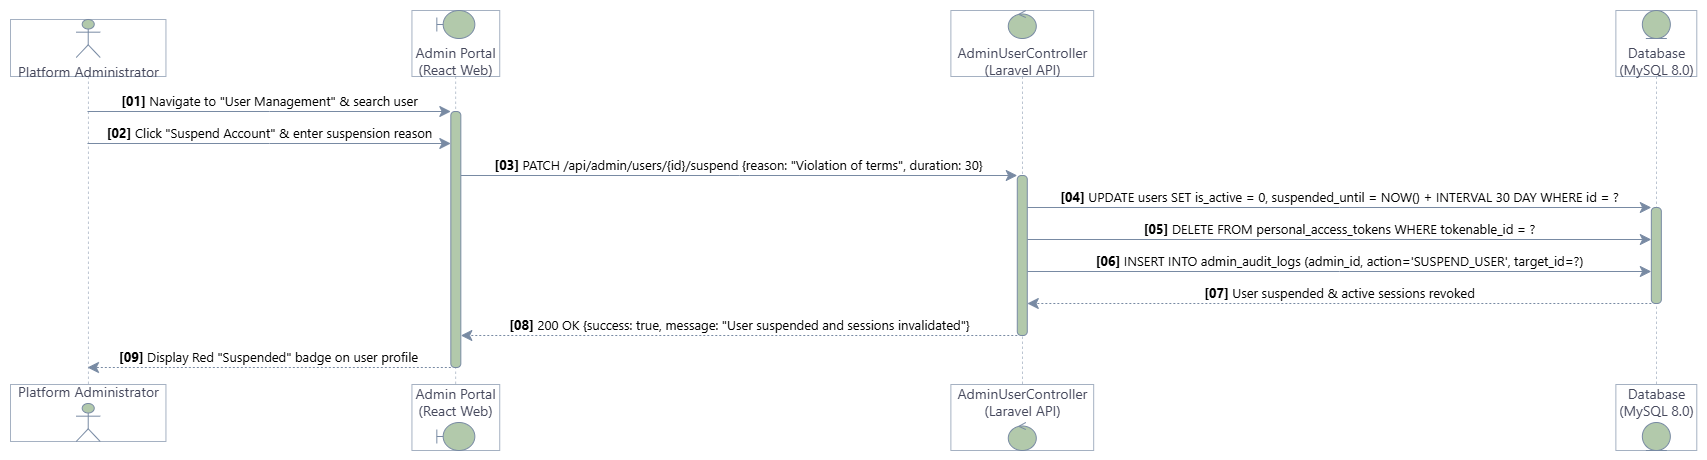
\includegraphics[width=0.75\linewidth]{figures/ssd_14.png}
\caption{Moderate User Accounts and Suspensions Sequence Diagram}
\label{fig:ssd14}
\end{figure}

\subsection{SSD-15: View System Analytics and Audit Logs}
As described in Figure \ref{fig:ssd15}, platform administrators inspect global operational analytics and audit logs through the administrative dashboard. The client sends an authenticated GET request to \texttt{/api/admin/analytics}. The backend queries aggregate statistics across \texttt{users}, \texttt{companies}, \texttt{job\_postings}, and \texttt{applications}, and fetches recent administrative event logs. The backend formats metrics---including daily registration velocity, active job counts, application submission volume, average ATS match scores, and domain verification turnaround times---into a structured JSON response. The client renders interactive charts and data tables for executive oversight.

\begin{figure}[H]
\centering
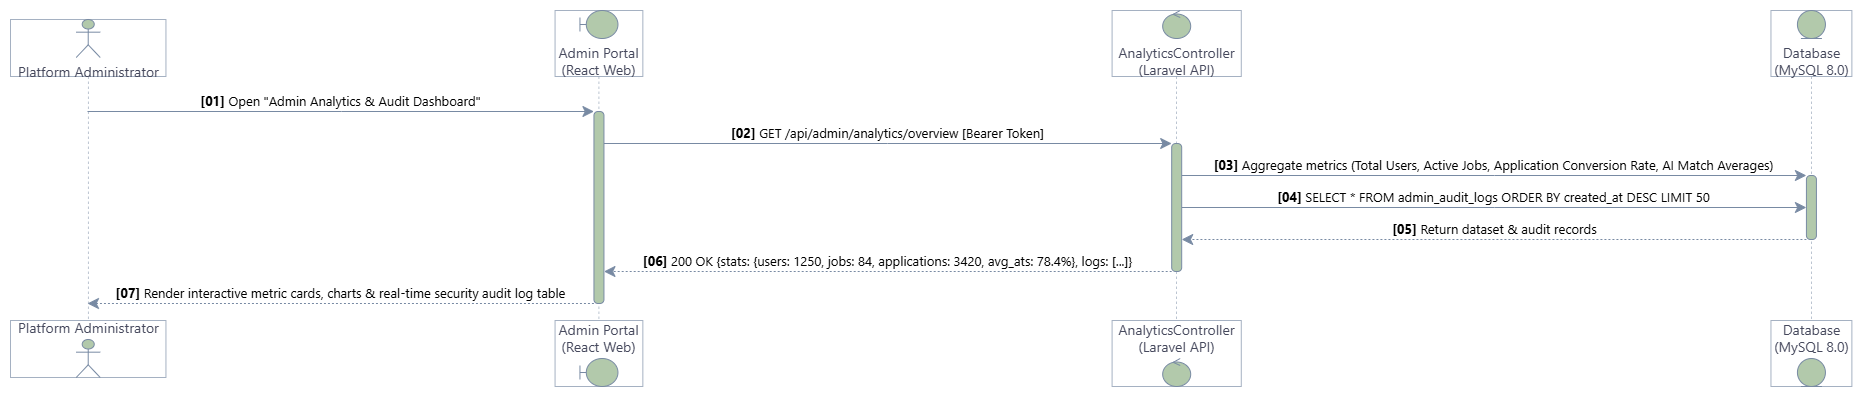
\includegraphics[width=0.75\linewidth]{figures/ssd_15.png}
\caption{View System Analytics and Audit Logs Sequence Diagram}
\label{fig:ssd15}
\end{figure}

\subsection{SSD-16: Update Profile and Professional Summary}
As described in Figure \ref{fig:ssd16}, a job seeker updates their personal profile information, headline, contact number, bio, and career experience records. The user edits profile fields in the settings workspace and submits changes. The client sends an HTTP PUT request to \texttt{/api/profile}. The backend validates input formats, updates the candidate record in \texttt{job\_seekers}, updates work history in \texttt{job\_experiences}, and returns the updated profile object. The client updates local cached state and displays a confirmation toast notification to the candidate.

\begin{figure}[H]
\centering
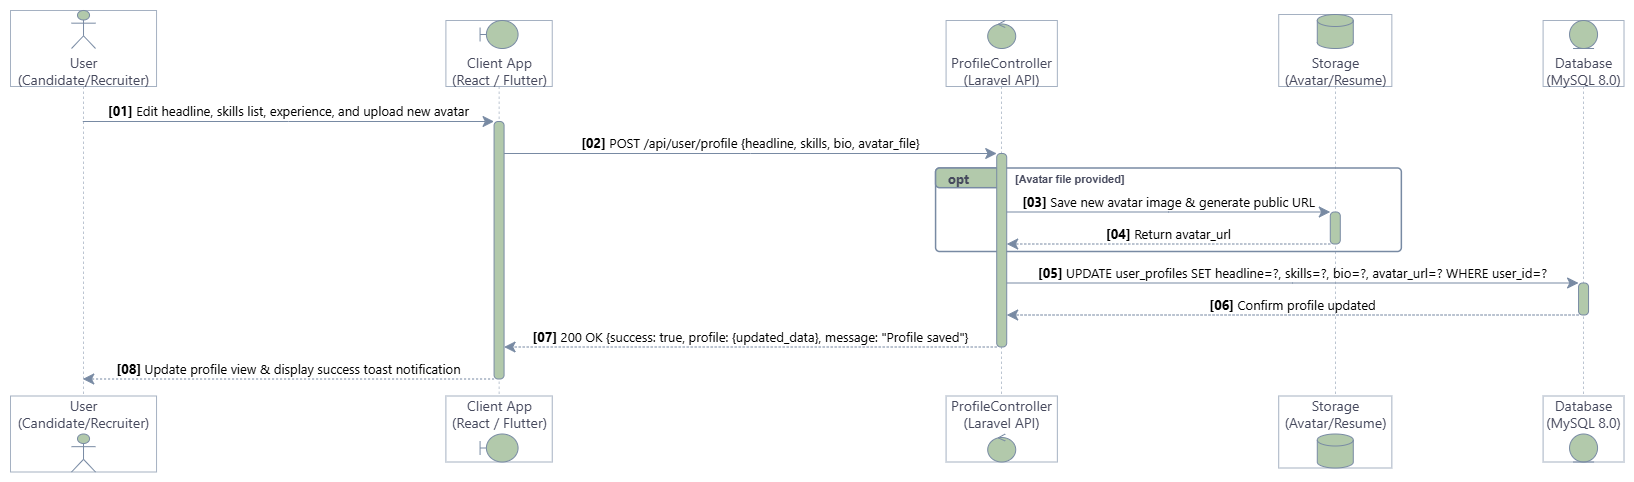
\includegraphics[width=0.75\linewidth]{figures/ssd_16.png}
\caption{Update Profile and Professional Summary Sequence Diagram}
\label{fig:ssd16}
\end{figure}

\subsection{SSD-17: Report Suspicious or Fraudulent Job Posting}
As described in Figure \ref{fig:ssd17}, a user reports a misleading, fraudulent, or non-compliant job listing directly from the vacancy details screen. The user selects a report category (e.g., Phishing Scam, Inaccurate Salary, Discriminatory Content), enters supporting details, and clicks submit. The client sends an HTTP POST request to \texttt{/api/jobs/\{id\}/report}. The backend authenticates the user, sanitizes comments, inserts a report ticket into the moderation queue, and returns an acknowledgment response. The job card indicates that the listing has been reported, and the ticket appears on the administrator moderation board.

\begin{figure}[H]
\centering
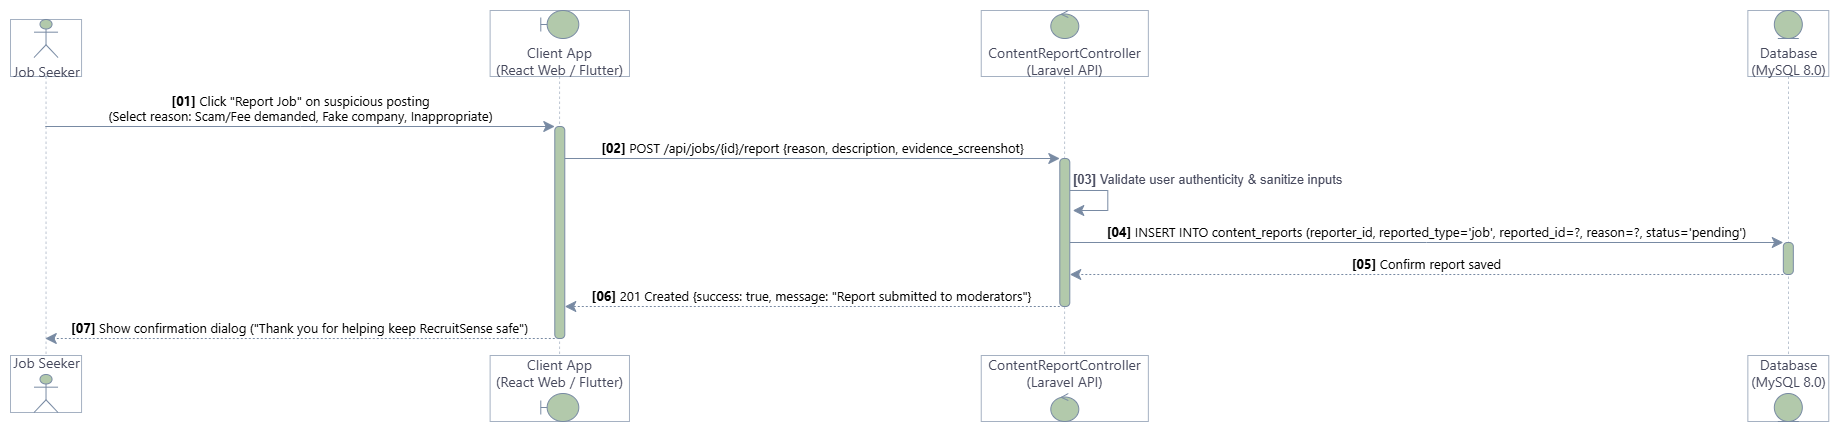
\includegraphics[width=0.75\linewidth]{figures/ssd_17.png}
\caption{Report Suspicious or Fraudulent Job Posting Sequence Diagram}
\label{fig:ssd17}
\end{figure}

\subsection{SSD-18: Review Reported Content and Fraud Claims}
As described in Figure \ref{fig:ssd18}, an administrator investigates reported job listings and user disputes from the moderation queue. The administrator retrieves open reports via a GET request to \texttt{/api/admin/reports}, inspects the flagged job listing and user comments, and executes an enforcement decision (Dismiss Report, Edit Job, or Remove Listing and Suspend Employer). The client dispatches a POST request to \texttt{/api/admin/reports/\{id\}/resolve}. The backend updates the report status, takes the corresponding action on the target job or user, and logs the administrative resolution in the audit log.

\begin{figure}[H]
\centering
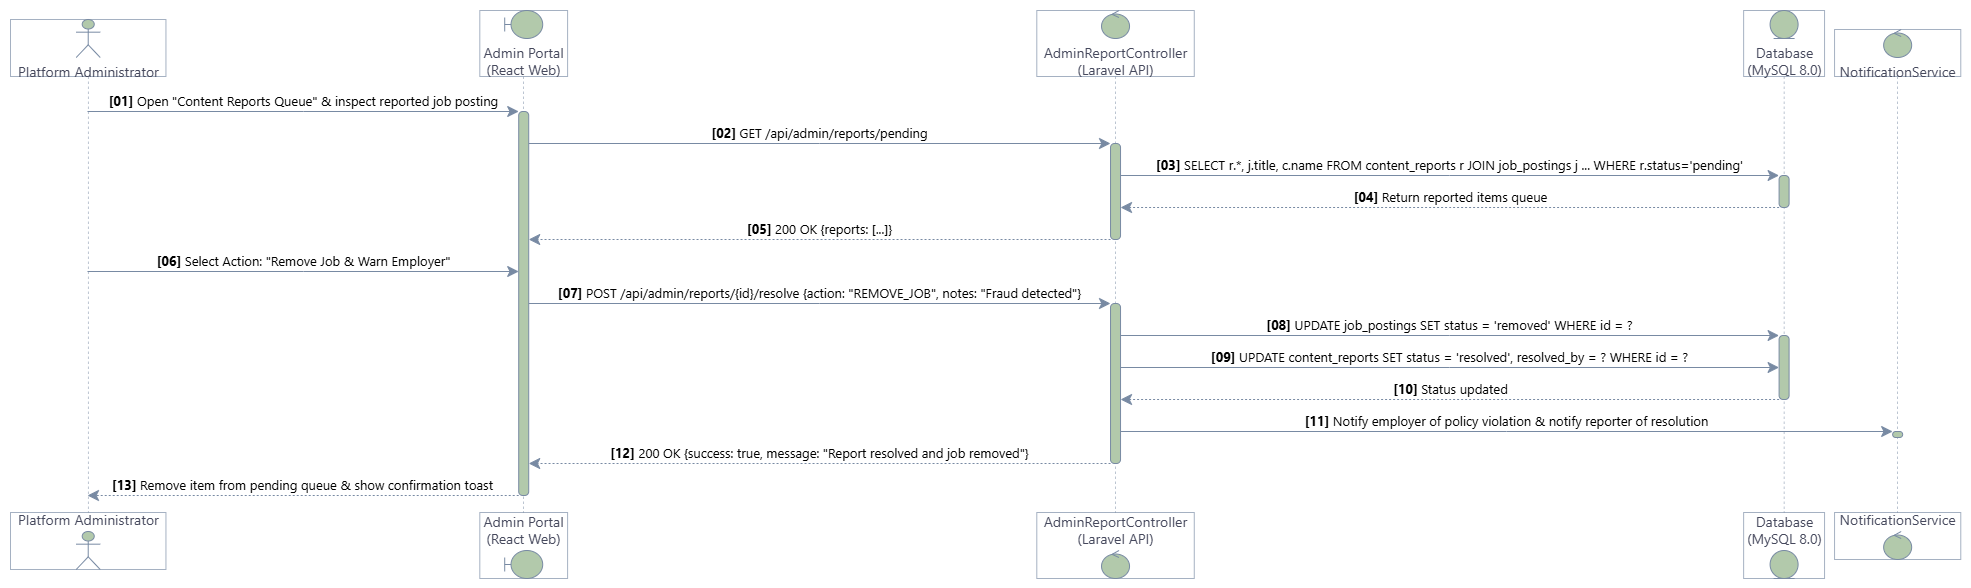
\includegraphics[width=0.75\linewidth]{figures/ssd_18.png}
\caption{Review Reported Content and Fraud Claims Sequence Diagram}
\label{fig:ssd18}
\end{figure}

\subsection{SSD-19: Skill Gap Course Recommendations and Feedback}
As described in Figure \ref{fig:ssd19}, following resume screening or during profile exploration, the candidate accesses personalized skill gap feedback. The client requests skill gap analytics for an application via GET \texttt{/api/applications/\{id\}/skill-gaps}. The backend queries the \texttt{skill\_gaps} table, retrieving matched skills, missing technical competencies, and curated course recommendations generated by the AI microservice. The client renders interactive skill chips---color-coded green for matched competencies and amber for missing areas---alongside direct links to recommended online courses and certifications to assist the candidate in upskilling.

\begin{figure}[H]
\centering
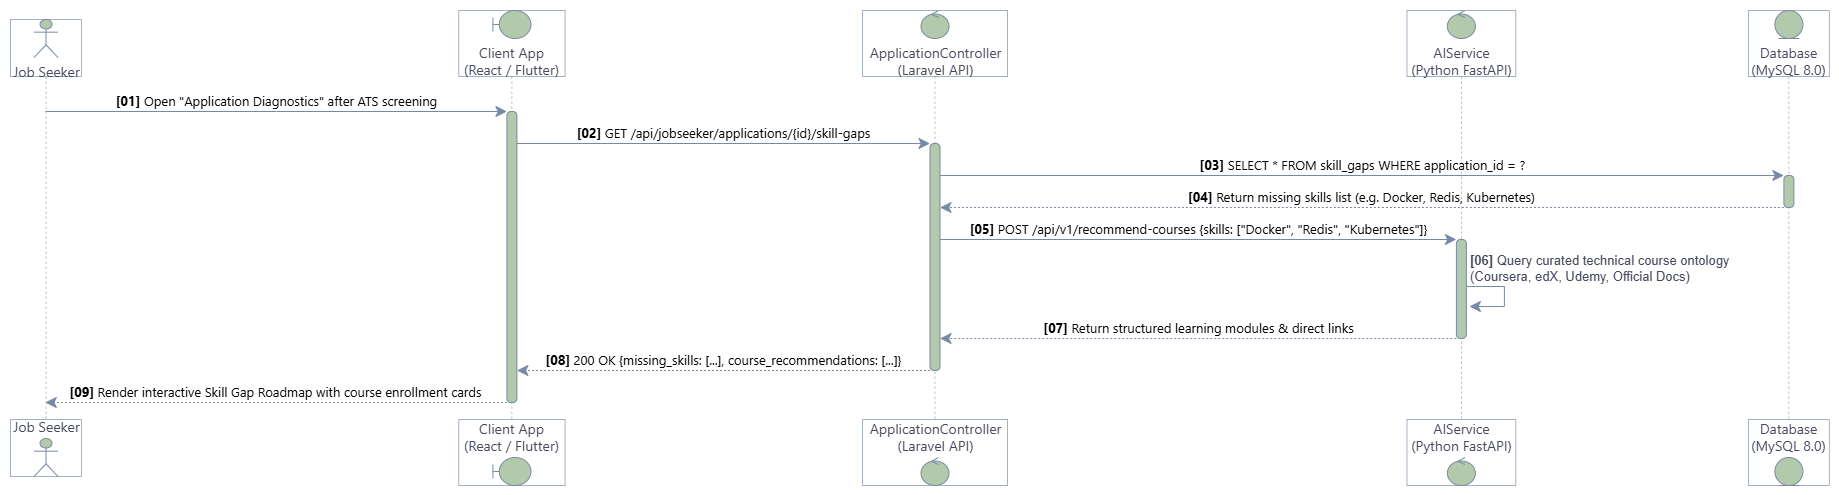
\includegraphics[width=0.75\linewidth]{figures/ssd_19.png}
\caption{Skill Gap Course Recommendations and Feedback Sequence Diagram}
\label{fig:ssd19}
\end{figure}

\subsection{SSD-20: Dynamic AI Assessment Quiz Generation}
As described in Figure \ref{fig:ssd20}, when a recruiter enables pre-screening assessments or a candidate opts to validate their skills, the system dynamically synthesizes a technical quiz. The client sends a request to \texttt{/api/jobs/\{id\}/generate-quiz}. The Laravel backend forwards the job title, required skill taxonomy, and difficulty level to the FastAPI AI microservice endpoint \texttt{/api/v1/generate-quiz}. The AI microservice constructs a structured prompt, queries the local LLM inference engine, and generates a structured JSON quiz comprising multiple-choice questions, answer options, and explanation metadata. The backend caches the quiz and delivers it to the candidate interface. Upon completion, answers are scored automatically, and the resulting assessment score is linked to the candidate's application record.

\begin{figure}[H]
\centering
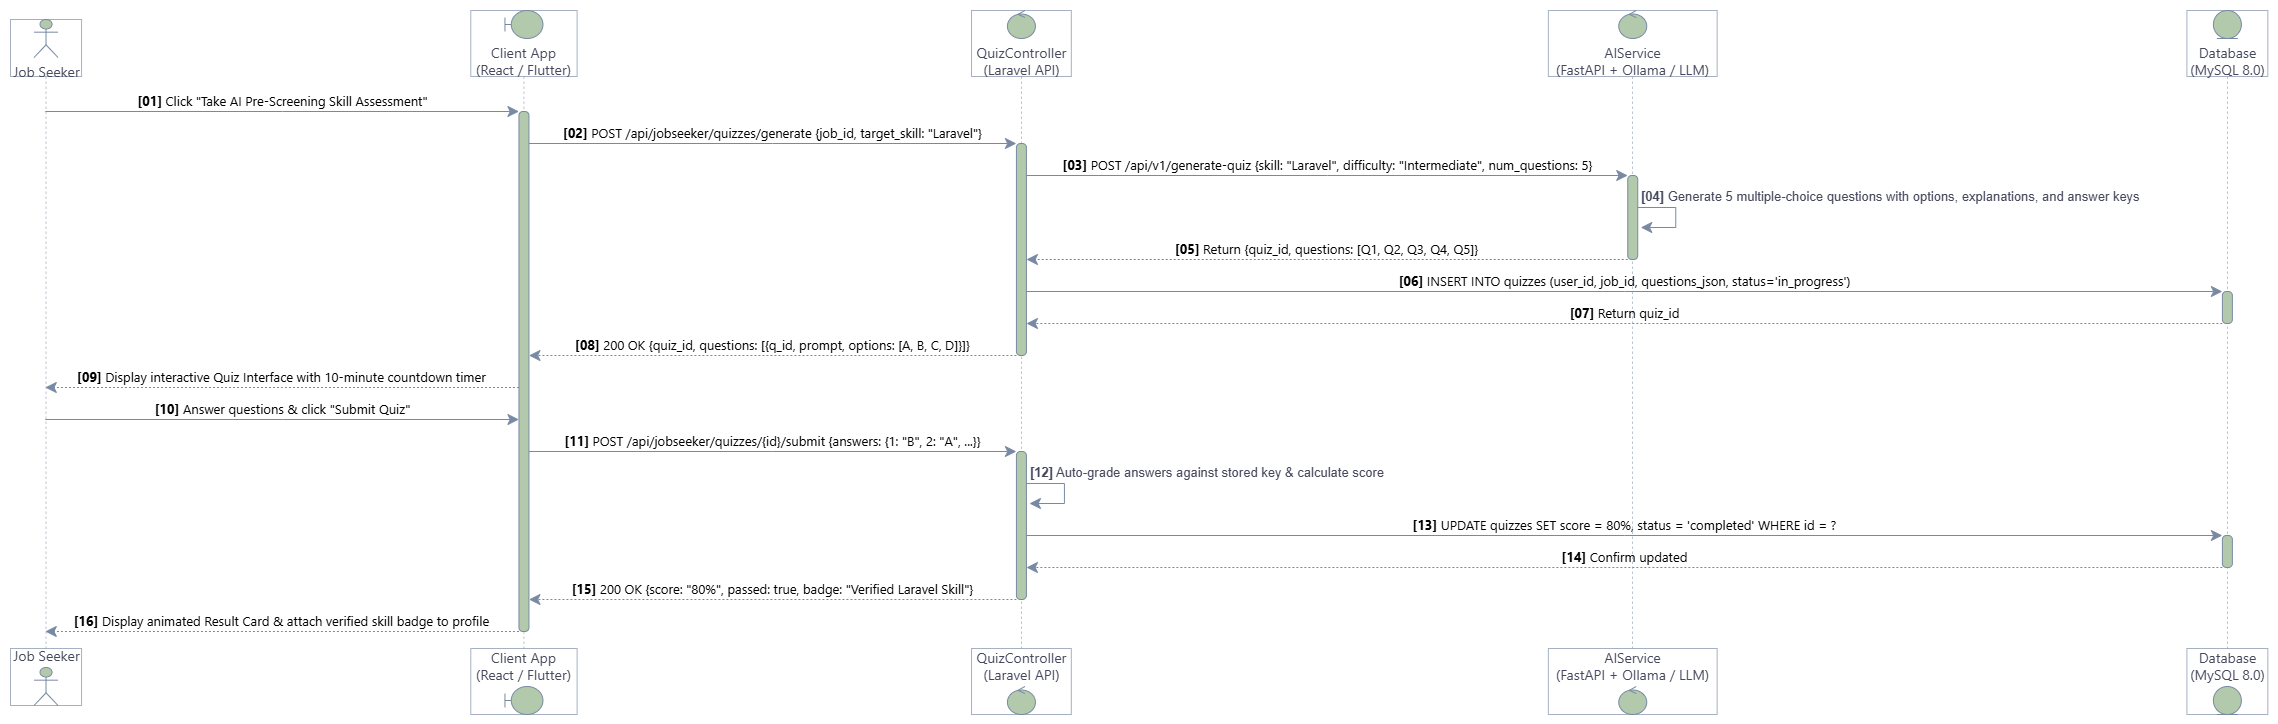
\includegraphics[width=0.75\linewidth]{figures/ssd_20.png}
\caption{Dynamic AI Assessment Quiz Generation Sequence Diagram}
\label{fig:ssd20}
\end{figure}

\section{Database Design}
The data layer of RecruitSense is built on a normalized relational schema in MySQL 8.0 following third normal form (3NF) principles, complemented by disk-backed ChromaDB vector collections for high-dimensional semantic search.

\subsection{Entity-Relationship (ER) Diagram}
Figure \ref{fig:erd_diagram} illustrates the complete Entity-Relationship diagram, specifying cardinalities, primary keys, and foreign key relationships across core database entities.

\begin{figure}[H]
\centering
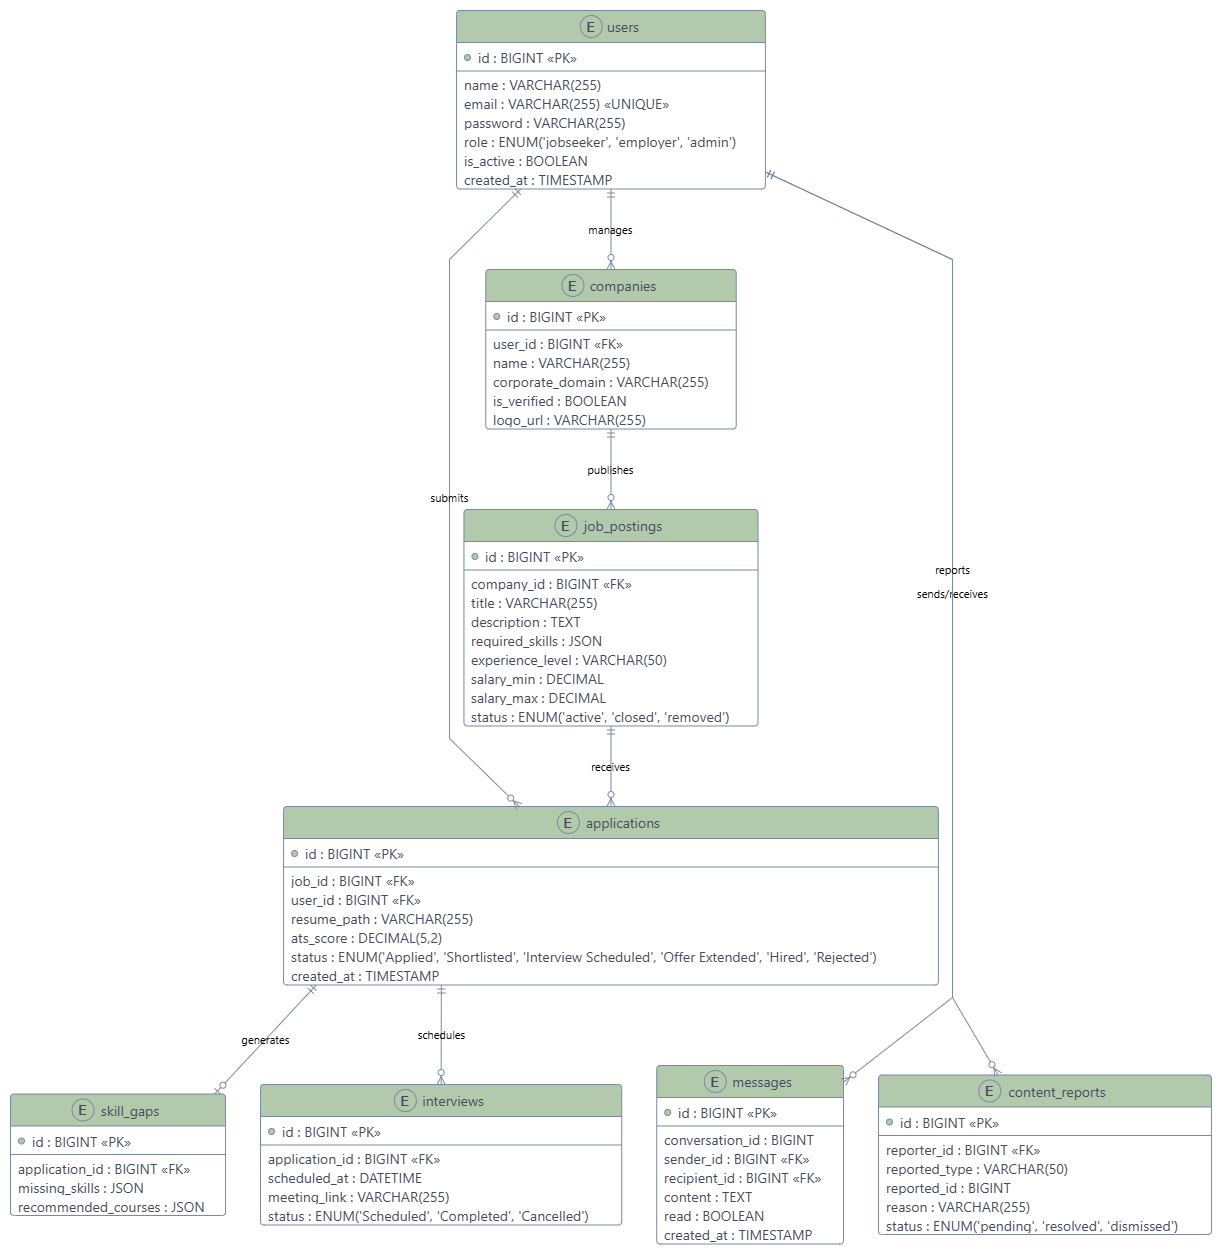
\includegraphics[width=0.85\linewidth]{figures/erd_diagram.png}
\caption{Entity-Relationship (ER) Diagram of RecruitSense Database Schema}
\label{fig:erd_diagram}
\end{figure}

\subsection{Complete Table Inventory and Data Dictionary}
The RecruitSense relational database consists of 14 core tables. The following data dictionaries provide complete field specifications, data types, constraints, and descriptions for every table in the schema.

\subsubsection{Table 1: \texttt{users}}
\begin{table}[H]
\centering
\small
\caption{Users Schema (\texttt{users})}
\label{tab:schema_users}
\begin{tabular}{|p{3cm}|p{2.8cm}|p{2.2cm}|p{5.5cm}|}
\hline
\textbf{Field Name} & \textbf{Type} & \textbf{Constraints} & \textbf{Description} \\ \hline
\texttt{id} & BIGINT UNSIGNED & PK, Auto-Inc & Unique user identifier \\ \hline
\texttt{name} & VARCHAR(255) & NOT NULL & Full legal name of user \\ \hline
\texttt{email} & VARCHAR(255) & NOT NULL, UNIQUE & Account login email address \\ \hline
\texttt{password} & VARCHAR(255) & NOT NULL & Bcrypt-hashed password string \\ \hline
\texttt{role} & ENUM & NOT NULL & \texttt{'job\_seeker'}, \texttt{'company'}, \texttt{'admin'} \\ \hline
\texttt{status} & VARCHAR(50) & Default: 'active' & Account status (\texttt{active}, \texttt{suspended}) \\ \hline
\texttt{avatar} & VARCHAR(255) & NULL & Profile avatar image URL / path \\ \hline
\texttt{created\_at} & TIMESTAMP & NULL & Account registration timestamp \\ \hline
\texttt{updated\_at} & TIMESTAMP & NULL & Last profile update timestamp \\ \hline
\end{tabular}
\end{table}

\subsubsection{Table 2: \texttt{companies}}
\begin{table}[H]
\centering
\small
\caption{Companies Schema (\texttt{companies})}
\label{tab:schema_companies}
\begin{tabular}{|p{3cm}|p{2.8cm}|p{2.2cm}|p{5.5cm}|}
\hline
\textbf{Field Name} & \textbf{Type} & \textbf{Constraints} & \textbf{Description} \\ \hline
\texttt{id} & BIGINT UNSIGNED & PK, Auto-Inc & Unique company identifier \\ \hline
\texttt{user\_id} & BIGINT UNSIGNED & FK \texttt{users.id} & Reference to parent owner user \\ \hline
\texttt{company\_name} & VARCHAR(255) & NOT NULL & Official registered corporate name \\ \hline
\texttt{domain} & VARCHAR(255) & NOT NULL & Corporate email domain \\ \hline
\texttt{website} & VARCHAR(255) & NULL & Official corporate website URL \\ \hline
\texttt{industry} & VARCHAR(255) & NULL & Business industry / sector \\ \hline
\texttt{location} & VARCHAR(255) & NULL & Company headquarters location \\ \hline
\texttt{verified} & BOOLEAN & Default: 0 & Domain verification status flag \\ \hline
\texttt{created\_at} & TIMESTAMP & NULL & Company profile creation timestamp \\ \hline
\texttt{updated\_at} & TIMESTAMP & NULL & Company profile update timestamp \\ \hline
\end{tabular}
\end{table}

\subsubsection{Table 3: \texttt{job\_seekers}}
\begin{table}[H]
\centering
\small
\caption{Job Seekers Schema (\texttt{job\_seekers})}
\label{tab:schema_job_seekers}
\begin{tabular}{|p{3cm}|p{2.8cm}|p{2.2cm}|p{5.5cm}|}
\hline
\textbf{Field Name} & \textbf{Type} & \textbf{Constraints} & \textbf{Description} \\ \hline
\texttt{id} & BIGINT UNSIGNED & PK, Auto-Inc & Unique candidate profile identifier \\ \hline
\texttt{user\_id} & BIGINT UNSIGNED & FK \texttt{users.id} & Reference to parent user record \\ \hline
\texttt{phone} & VARCHAR(50) & NULL & Primary contact telephone number \\ \hline
\texttt{headline} & VARCHAR(255) & NULL & Professional headline / title \\ \hline
\texttt{summary} & TEXT & NULL & Career bio and executive summary \\ \hline
\texttt{location} & VARCHAR(255) & NULL & Current city and country of residence \\ \hline
\texttt{skills} & TEXT & NULL & Comma-separated candidate skills \\ \hline
\texttt{experience\_years}& INT & Default: 0 & Total cumulative years of experience \\ \hline
\texttt{created\_at} & TIMESTAMP & NULL & Profile creation timestamp \\ \hline
\texttt{updated\_at} & TIMESTAMP & NULL & Profile update timestamp \\ \hline
\end{tabular}
\end{table}

\subsubsection{Table 4: \texttt{job\_postings}}
\begin{table}[H]
\centering
\small
\caption{Job Postings Schema (\texttt{job\_postings})}
\label{tab:schema_job_postings}
\begin{tabular}{|p{3cm}|p{2.8cm}|p{2.2cm}|p{5.5cm}|}
\hline
\textbf{Field Name} & \textbf{Type} & \textbf{Constraints} & \textbf{Description} \\ \hline
\texttt{id} & BIGINT UNSIGNED & PK, Auto-Inc & Unique job vacancy identifier \\ \hline
\texttt{company\_id} & BIGINT UNSIGNED & FK \texttt{companies.id} & Reference to hiring organization \\ \hline
\texttt{title} & VARCHAR(255) & NOT NULL & Job vacancy title \\ \hline
\texttt{department} & VARCHAR(255) & NULL & Department / team category \\ \hline
\texttt{job\_type} & ENUM & NOT NULL & \texttt{'Full-Time'}, \texttt{'Part-Time'}, \texttt{'Remote'}, \dots \\ \hline
\texttt{description} & TEXT & NOT NULL & Full job description and duties \\ \hline
\texttt{required\_skills}& TEXT & NOT NULL & Comma-separated required skill tags \\ \hline
\texttt{salary\_min} & DECIMAL(10,2) & NULL & Minimum compensation range \\ \hline
\texttt{salary\_max} & DECIMAL(10,2) & NULL & Maximum compensation range \\ \hline
\texttt{status} & VARCHAR(50) & Default: 'active' & Vacancy state (\texttt{active}, \texttt{draft}, \texttt{closed}) \\ \hline
\texttt{created\_at} & TIMESTAMP & NULL & Job posting publication timestamp \\ \hline
\texttt{updated\_at} & TIMESTAMP & NULL & Job posting modification timestamp \\ \hline
\end{tabular}
\end{table}

\subsubsection{Table 5: \texttt{resumes}}
\begin{table}[H]
\centering
\small
\caption{Resumes Schema (\texttt{resumes})}
\label{tab:schema_resumes}
\begin{tabular}{|p{3cm}|p{2.8cm}|p{2.2cm}|p{5.5cm}|}
\hline
\textbf{Field Name} & \textbf{Type} & \textbf{Constraints} & \textbf{Description} \\ \hline
\texttt{id} & BIGINT UNSIGNED & PK, Auto-Inc & Unique resume document identifier \\ \hline
\texttt{job\_seeker\_id} & BIGINT UNSIGNED & FK \texttt{job\_seekers.id} & Reference to candidate profile \\ \hline
\texttt{file\_name} & VARCHAR(255) & NOT NULL & Original uploaded file name \\ \hline
\texttt{file\_path} & VARCHAR(255) & NOT NULL & Obfuscated file path on disk \\ \hline
\texttt{extracted\_text}& LONGTEXT & NULL & Parsed plain text layer from PDF \\ \hline
\texttt{parsed\_skills} & JSON & NULL & JSON array of recognized skills \\ \hline
\texttt{is\_primary} & BOOLEAN & Default: 1 & Primary active resume flag \\ \hline
\texttt{created\_at} & TIMESTAMP & NULL & Resume upload timestamp \\ \hline
\texttt{updated\_at} & TIMESTAMP & NULL & Resume parsing timestamp \\ \hline
\end{tabular}
\end{table}

\subsubsection{Table 6: \texttt{applications}}
\begin{table}[H]
\centering
\small
\caption{Applications Schema (\texttt{applications})}
\label{tab:schema_applications}
\begin{tabular}{|p{3cm}|p{2.8cm}|p{2.2cm}|p{5.5cm}|}
\hline
\textbf{Field Name} & \textbf{Type} & \textbf{Constraints} & \textbf{Description} \\ \hline
\texttt{id} & BIGINT UNSIGNED & PK, Auto-Inc & Unique application identifier \\ \hline
\texttt{job\_posting\_id}& BIGINT UNSIGNED & FK \texttt{job\_postings.id}& Reference to target job vacancy \\ \hline
\texttt{job\_seeker\_id} & BIGINT UNSIGNED & FK \texttt{job\_seekers.id} & Reference to applicant candidate \\ \hline
\texttt{resume\_path} & VARCHAR(255) & NOT NULL & Stored PDF resume file path \\ \hline
\texttt{ats\_score} & DECIMAL(5,2) & NOT NULL & Computed overall ATS match score \% \\ \hline
\texttt{status} & VARCHAR(50) & Default: 'applied' & Pipeline stage (\texttt{applied}, \texttt{screening}, \dots) \\ \hline
\texttt{interview\_at} & DATETIME & NULL & Scheduled interview date/time \\ \hline
\texttt{notes} & TEXT & NULL & Recruiter internal evaluation notes \\ \hline
\texttt{created\_at} & TIMESTAMP & NULL & Application submission timestamp \\ \hline
\texttt{updated\_at} & TIMESTAMP & NULL & Application status update timestamp \\ \hline
\end{tabular}
\end{table}

\subsubsection{Table 7: \texttt{skill\_gaps}}
\begin{table}[H]
\centering
\small
\caption{Skill Gaps Schema (\texttt{skill\_gaps})}
\label{tab:schema_skill_gaps}
\begin{tabular}{|p{3cm}|p{2.8cm}|p{2.2cm}|p{5.5cm}|}
\hline
\textbf{Field Name} & \textbf{Type} & \textbf{Constraints} & \textbf{Description} \\ \hline
\texttt{id} & BIGINT UNSIGNED & PK, Auto-Inc & Unique skill gap record identifier \\ \hline
\texttt{application\_id} & BIGINT UNSIGNED & FK \texttt{applications.id}& Reference to candidate application \\ \hline
\texttt{matched\_skills} & JSON & NOT NULL & JSON array of matched skill strings \\ \hline
\texttt{missing\_skills} & JSON & NOT NULL & JSON array of missing required skills \\ \hline
\texttt{bonus\_skills} & JSON & NULL & JSON array of additional candidate skills \\ \hline
\texttt{course\_recommendations}& JSON & NULL & JSON array of recommended course objects \\ \hline
\texttt{created\_at} & TIMESTAMP & NULL & Diagnostic generation timestamp \\ \hline
\texttt{updated\_at} & TIMESTAMP & NULL & Last update timestamp \\ \hline
\end{tabular}
\end{table}

\subsubsection{Table 8: \texttt{conversations}}
\begin{table}[H]
\centering
\small
\caption{Conversations Schema (\texttt{conversations})}
\label{tab:schema_conversations}
\begin{tabular}{|p{3cm}|p{2.8cm}|p{2.2cm}|p{5.5cm}|}
\hline
\textbf{Field Name} & \textbf{Type} & \textbf{Constraints} & \textbf{Description} \\ \hline
\texttt{id} & BIGINT UNSIGNED & PK, Auto-Inc & Unique conversation thread ID \\ \hline
\texttt{job\_seeker\_user\_id}& BIGINT UNSIGNED & FK \texttt{users.id} & Candidate user identifier \\ \hline
\texttt{company\_user\_id} & BIGINT UNSIGNED & FK \texttt{users.id} & Recruiter user identifier \\ \hline
\texttt{last\_message\_at} & TIMESTAMP & NULL & Timestamp of most recent message \\ \hline
\texttt{created\_at} & TIMESTAMP & NULL & Thread creation timestamp \\ \hline
\texttt{updated\_at} & TIMESTAMP & NULL & Thread update timestamp \\ \hline
\end{tabular}
\end{table}

\subsubsection{Table 9: \texttt{messages}}
\begin{table}[H]
\centering
\small
\caption{Messages Schema (\texttt{messages})}
\label{tab:schema_messages}
\begin{tabular}{|p{3cm}|p{2.8cm}|p{2.2cm}|p{5.5cm}|}
\hline
\textbf{Field Name} & \textbf{Type} & \textbf{Constraints} & \textbf{Description} \\ \hline
\texttt{id} & BIGINT UNSIGNED & PK, Auto-Inc & Unique message identifier \\ \hline
\texttt{conversation\_id}& BIGINT UNSIGNED & FK \texttt{conversations.id}& Parent conversation thread \\ \hline
\texttt{sender\_id} & BIGINT UNSIGNED & FK \texttt{users.id} & User ID of message author \\ \hline
\texttt{message} & TEXT & NOT NULL & Text content of message \\ \hline
\texttt{is\_read} & BOOLEAN & Default: 0 & Message read acknowledgment flag \\ \hline
\texttt{created\_at} & TIMESTAMP & NULL & Message transmission timestamp \\ \hline
\texttt{updated\_at} & TIMESTAMP & NULL & Message update timestamp \\ \hline
\end{tabular}
\end{table}

\subsubsection{Table 10: \texttt{notifications}}
\begin{table}[H]
\centering
\small
\caption{Notifications Schema (\texttt{notifications})}
\label{tab:schema_notifications}
\begin{tabular}{|p{3cm}|p{2.8cm}|p{2.2cm}|p{5.5cm}|}
\hline
\textbf{Field Name} & \textbf{Type} & \textbf{Constraints} & \textbf{Description} \\ \hline
\texttt{id} & BIGINT UNSIGNED & PK, Auto-Inc & Unique notification identifier \\ \hline
\texttt{user\_id} & BIGINT UNSIGNED & FK \texttt{users.id} & Target recipient user ID \\ \hline
\texttt{type} & VARCHAR(255) & NOT NULL & Notification category event \\ \hline
\texttt{title} & VARCHAR(255) & NOT NULL & Notification summary headline \\ \hline
\texttt{message} & TEXT & NOT NULL & Detailed notification text \\ \hline
\texttt{read\_at} & TIMESTAMP & NULL & Read timestamp (NULL if unread) \\ \hline
\texttt{created\_at} & TIMESTAMP & NULL & Notification dispatch timestamp \\ \hline
\texttt{updated\_at} & TIMESTAMP & NULL & Notification update timestamp \\ \hline
\end{tabular}
\end{table}

\subsubsection{Table 11: \texttt{saved\_jobs}}
\begin{table}[H]
\centering
\small
\caption{Saved Jobs Schema (\texttt{saved\_jobs})}
\label{tab:schema_saved_jobs}
\begin{tabular}{|p{3cm}|p{2.8cm}|p{2.2cm}|p{5.5cm}|}
\hline
\textbf{Field Name} & \textbf{Type} & \textbf{Constraints} & \textbf{Description} \\ \hline
\texttt{id} & BIGINT UNSIGNED & PK, Auto-Inc & Unique bookmark identifier \\ \hline
\texttt{user\_id} & BIGINT UNSIGNED & FK \texttt{users.id} & Candidate user identifier \\ \hline
\texttt{job\_posting\_id}& BIGINT UNSIGNED & FK \texttt{job\_postings.id}& Bookmarked vacancy identifier \\ \hline
\texttt{created\_at} & TIMESTAMP & NULL & Bookmark creation timestamp \\ \hline
\texttt{updated\_at} & TIMESTAMP & NULL & Bookmark update timestamp \\ \hline
\end{tabular}
\end{table}

\subsubsection{Table 12: \texttt{posts}}
\begin{table}[H]
\centering
\small
\caption{Community Posts Schema (\texttt{posts})}
\label{tab:schema_posts}
\begin{tabular}{|p{3cm}|p{2.8cm}|p{2.2cm}|p{5.5cm}|}
\hline
\textbf{Field Name} & \textbf{Type} & \textbf{Constraints} & \textbf{Description} \\ \hline
\texttt{id} & BIGINT UNSIGNED & PK, Auto-Inc & Unique post identifier \\ \hline
\texttt{user\_id} & BIGINT UNSIGNED & FK \texttt{users.id} & Author user identifier \\ \hline
\texttt{content} & TEXT & NOT NULL & Text content of community post \\ \hline
\texttt{image\_url} & VARCHAR(255) & NULL & Attached media image URL \\ \hline
\texttt{likes\_count} & INT & Default: 0 & Aggregate like count \\ \hline
\texttt{created\_at} & TIMESTAMP & NULL & Post publication timestamp \\ \hline
\texttt{updated\_at} & TIMESTAMP & NULL & Post modification timestamp \\ \hline
\end{tabular}
\end{table}

\subsubsection{Table 13: \texttt{job\_experiences}}
\begin{table}[H]
\centering
\small
\caption{Job Experiences Schema (\texttt{job\_experiences})}
\label{tab:schema_job_experiences}
\begin{tabular}{|p{3cm}|p{2.8cm}|p{2.2cm}|p{5.5cm}|}
\hline
\textbf{Field Name} & \textbf{Type} & \textbf{Constraints} & \textbf{Description} \\ \hline
\texttt{id} & BIGINT UNSIGNED & PK, Auto-Inc & Unique experience record ID \\ \hline
\texttt{job\_seeker\_id} & BIGINT UNSIGNED & FK \texttt{job\_seekers.id} & Candidate profile reference \\ \hline
\texttt{company\_name} & VARCHAR(255) & NOT NULL & Employing organization name \\ \hline
\texttt{position} & VARCHAR(255) & NOT NULL & Job title / designation \\ \hline
\texttt{start\_date} & DATE & NOT NULL & Employment commencement date \\ \hline
\texttt{end\_date} & DATE & NULL & Employment conclusion date (NULL if current) \\ \hline
\texttt{is\_current} & BOOLEAN & Default: 0 & Currently employed flag \\ \hline
\texttt{description} & TEXT & NULL & Role responsibilities summary \\ \hline
\texttt{created\_at} & TIMESTAMP & NULL & Experience record creation date \\ \hline
\texttt{updated\_at} & TIMESTAMP & NULL & Experience record update date \\ \hline
\end{tabular}
\end{table}

\subsubsection{Table 14: \texttt{admin\_settings}}
\begin{table}[H]
\centering
\small
\caption{Admin Settings Schema (\texttt{admin\_settings})}
\label{tab:schema_admin_settings}
\begin{tabular}{|p{3cm}|p{2.8cm}|p{2.2cm}|p{5.5cm}|}
\hline
\textbf{Field Name} & \textbf{Type} & \textbf{Constraints} & \textbf{Description} \\ \hline
\texttt{id} & BIGINT UNSIGNED & PK, Auto-Inc & Unique setting record identifier \\ \hline
\texttt{key} & VARCHAR(255) & NOT NULL, UNIQUE & Configuration key string \\ \hline
\texttt{value} & TEXT & NULL & Serialized configuration value \\ \hline
\texttt{description} & VARCHAR(255) & NULL & Functional description of setting \\ \hline
\texttt{created\_at} & TIMESTAMP & NULL & Setting creation timestamp \\ \hline
\texttt{updated\_at} & TIMESTAMP & NULL & Last modification timestamp \\ \hline
\end{tabular}
\end{table}

\section{GUI Design}
The user interface of RecruitSense is engineered for visual clarity, operational velocity, and responsive accessibility across web and mobile viewports.

\subsection{Job Seeker GUI Direction}
The job seeker interface emphasizes frictionless job exploration, clear application tracking, and transparent ATS feedback. Figure \ref{fig:gui_jobseeker_layout} illustrates the layout direction for candidate discovery and application screens.

\begin{figure}[H]
\centering
\fbox{\parbox[c][6.5cm][c]{0.88\linewidth}{\centering \textbf{GUI Wireframe / Layout Placeholder: Job Seeker Interface}\\\vspace{3mm}\small\textit{Reserved area for Job Discovery, Resume Submission, and ATS Feedback Screen Layouts}}}
\caption{Job Seeker GUI Layout Direction (Web and Mobile)}
\label{fig:gui_jobseeker_layout}
\end{figure}

\subsection{Recruiter GUI Direction}
The recruiter interface centers on job vacancy publication, automated candidate ranking sorted by ATS match percentage, stage-by-stage pipeline Kanban progression, and conversational Candidate RAG exploration. Figure \ref{fig:gui_recruiter_layout} shows the recruiter interface layout direction.

\begin{figure}[H]
\centering
\fbox{\parbox[c][6.5cm][c]{0.88\linewidth}{\centering \textbf{GUI Wireframe / Layout Placeholder: Recruiter Interface}\\\vspace{3mm}\small\textit{Reserved area for Candidate Ranking, Pipeline Kanban, and Candidate RAG Dialog Layouts}}}
\caption{Recruiter and Employer GUI Layout Direction}
\label{fig:gui_recruiter_layout}
\end{figure}

\subsection{Administrator GUI Direction}
The administrative interface provides unified visibility into platform operational metrics, corporate email domain verification queues, content moderation, and audit logs. Figure \ref{fig:gui_admin_layout} illustrates the administrator layout direction.

\begin{figure}[H]
\centering
\fbox{\parbox[c][6.5cm][c]{0.88\linewidth}{\centering \textbf{GUI Wireframe / Layout Placeholder: Administrator Console}\\\vspace{3mm}\small\textit{Reserved area for Domain Verification, Moderation, and Global Analytics Layouts}}}
\caption{Platform Administrator GUI Layout Direction}
\label{fig:gui_admin_layout}
\end{figure}

\section{External Interfaces and Deployment}
Figure \ref{fig:cicd_pipeline} illustrates the Continuous Integration and Deployment (CI/CD) and service interface model of RecruitSense.

\begin{figure}[H]
\centering
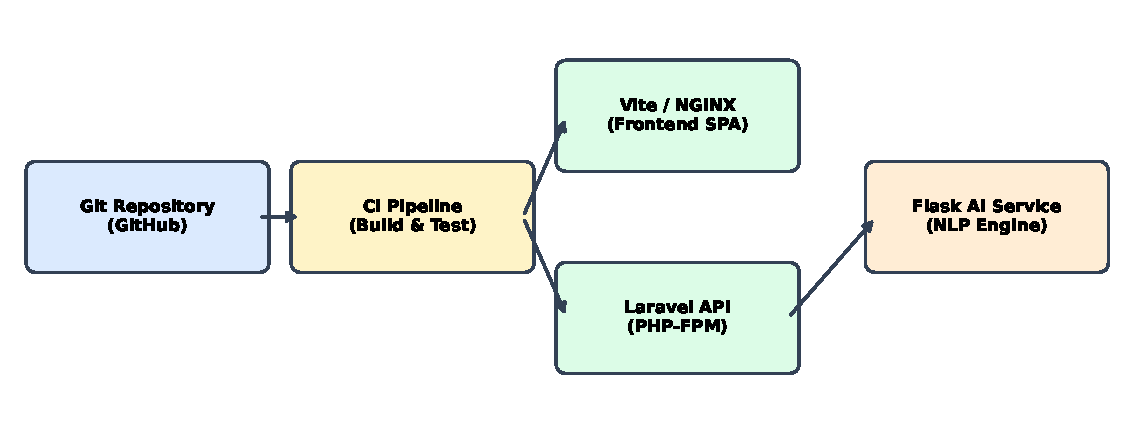
\includegraphics[width=0.8\linewidth]{figures/cicd_pipeline.pdf}
\caption{CI/CD and Service Deployment Pipeline of RecruitSense}
\label{fig:cicd_pipeline}
\end{figure}

\section{Chapter Summary}
This chapter presented the comprehensive system design of \textbf{RecruitSense}. It articulated the 4-tier decoupled architecture spanning React Web, Flutter Mobile, Laravel API, FastAPI AI, and ChromaDB vector persistence, analyzed technical and security design constraints, presented the state-machine methodology for candidate hiring pipelines, documented 20 System Sequence Diagrams (SSDs) covering all core operational workflows with detailed narrative explanations, specified the complete 14-table 3NF MySQL relational database schema and data dictionary, and outlined GUI directions and CI/CD deployment pipelines. This design provides the structural blueprint for the technical realization presented in Chapter \ref{chap:sysImplementation}.
